\documentclass[notes,tikz,minted]{agony}

\declaretheorem[name=Warm-Up Exercise,refname={WE,WEs},style=thmquoteresult,parent=chapter]{warmup}
\declaretheoremstyle[
	headfont=\bfseries\color{OliveGreen},
  notefont=\mdseries,
	bodyfont=\normalfont,
	mdframed={style=mdquote,linecolor=ForestGreen,backgroundcolor=ForestGreen!5},
]{thmquotegreen}
\declaretheorem[name=Recommended Problem,refname={RP,RPs},style=thmquotegreen,parent=chapter]{recommended}
\declaretheorem[name=Challenge,refname={C,Cs},style=thmquotered,parent=chapter]{challenge}

\title{MATH 135 Fall 2020: Extra Practice}
\author{James Ah Yong and contributors}
\begin{document}
\thispagestyle{firstpage}

\chapter*{MATH 135 Fall 2020:\\{\huge Extra Practice}}

\begin{mdframed}[style=mdround,linecolor=red,backgroundcolor=CarnationPink!5]
  This document was entirely written by then-first year Double Degrees.
  \textbf{\color{Red}{Nothing here is official. There are no guarantees that content is remotely close to correct.}}
  If you find a mistake, please either \href{https://agony.retrocraft.ca/#contact}{let me know}
  or make a \href{https://github.com/RetroCraft/problems/pulls}{pull request} fixing it.

  \textbf{\color{Red}{Try the problems first}} before looking at solutions.
  You won't learn by reading someone else's work.
\end{mdframed}

\begin{multicols*}{2}
  % Print ToC without ToC title
  \makeatletter
  \@starttoc{toc}
  \makeatother
\end{multicols*}

\chapter{Operating Systems Introduction}

\lecture{(05/09)}
Generally, an \term{operating system} acts partially as a cop (e.g., watching for unplugged USB drives)
and as a facilitator (e.g., allowing you to interface with any storage device with \verb|fopen|).
It is responsible for:
\begin{itemize}[nosep]
  \item managing resources;
  \item creating execution environments;
  \item loading programs; and
  \item providing common services and utilities
\end{itemize}
We will consider an OS from three views:
\begin{enumerate}[1.,nosep]
  \item Application: what does an OS provide?
        Provides an \term{execution environment}
        which provides resources, interfaces, and isolation.
  \item System: what problems does an OS solve?
        Manages hardware resources, allocates them to programs,
        and controls access to shared resources between programs.
  \item Implementation: how is an OS built?
        It must be \term[concurrency]{concurrent} (allow multiple things to run at once)
        and \term{real-time} (respond to events in a set time).
\end{enumerate}

\begin{defn}[kernel]
  The part of the operating system that responds to system calls,
  interrupts, and exceptions.
\end{defn}
\begin{defn}[operating system]
  Includes the kernel, but also other related programs that provide services
  for applications. For example, utility programs, command interpreters, and programming libraries.
\end{defn}

The kernel protects from bad \term{user programs} by isolating
them in \term{user space} (resp. \term{kernel space})
and allowing them only to interact with hardware using system calls.

\begin{defn}[system call]
  A user interaction with the OS.
  For example, the C function \verb|fopen| makes the Linux syscall
  \verb|sys_open|.
  They are much slower than calling a user function.
\end{defn}

\begin{defn*}[types of kernels]
  \begin{itemize}[nosep]
    \item \term[kernel!monolithic kernel]{Monolithic}:
          when the entire OS is the kernel (e.g. Linux)
    \item \term[kernel!microkernel]{Microkernel}:
          when only absolutely necessary parts are in the kernel
    \item \term[kernel!hybrid kernel]{Hybrid}:
          somewhere between monolithic kernels and microkernels (e.g. Windows, macOS)
    \item \term[real-time operating system]{Real-time}:
          with stringent event response time, guarantees, and scheduling
  \end{itemize}
\end{defn*}

A monolithic kernel is faster, since we avoid slower system calls.
However, they are less secure since third-party drivers must be trusted and included in the kernel.

\lecture{(05/11)}
Provided by the execution environment are abstract entities
that a program is able to manipulate:
\begin{itemize}[nosep]
  \item files and file systems (secondary storage; e.g. HDDs)
  \item address spaces (primary memory; RAM)
  \item processes, threads (program execution)
  \item sockets, pipes (message channels)
\end{itemize}

\chapter{Threads}

\begin{defn}[thread]
  Sequence of instructions
\end{defn}

An ordinary \term{sequential program} has only a single thread.
Analogous to how DFAs have a single state and NFAs can follow multiple paths,
a program can have multiple threads of execution.
The threads can be for the same role (e.g. one per server visitor)
or for different roles (e.g. Chrome's JavaScript and graphics engines).

Threads allow for:
\begin{itemize}[nosep]
  \item \term{concurrency}: allow multiple tasks to occur at once
  \item \term{parallelism}: different threads on different processors to increase throughput
  \item \term{responsiveness}: allow blocking tasks to not block the whole system
  \item \term{priority}: do things that are more important first
  \item \term{modularity}: separate out tasks into threads that can't crash each other
\end{itemize}
A thread will pause execution when it is \term[blocking]{blocked}.

Consider for example the traffic simulation for Assignment 1.
Each thread represents a vehicle passing through an intersection,
and we are trying to prevent collisions.

A thread can create a new thread using \verb|thread_fork|.
The original and new threads share global data and the heap.
However, the new thread has a separate, private stack.

For example, in \texttt{/kern/synchprobs/traffic.c}:
\begin{minted}{c}
  for (i = 0; i < NumThreads; i++) {
    error = thread_fork("vehicle_simulation thread", NULL, vehicle_simulation,
                        NULL, i);
    if (error) {
      panic("traffic_simulation: thread_fork failed: %s\n", strerror(error));
    }
  }
\end{minted}
we start a thread running \mintinline{c}{vehicle_simulation(NULL, i)}.

In OS/161, we create a thread with
\begin{minted}{c}
  int thread_fork(
    const char *name,
    struct proc *proc,
    void (*func)(void *, unsigned long),
    void *data1,
    unsigned long data2
  );
\end{minted}
and can terminate with \mintinline{c}{void thread_exit(void)}
and yield with \mintinline{c}{void thread_yield(void)}.
However, we cannot control the order that threads run in.

Recall from CS 241 how to execute a single thread:
fetch--execute cycle.
In CS 241, we called all the registers $\$0,\dotsc,\$31$.
In real life, they have names like a0 and s8.

CS 241 passed all arguments via the stack.
We will pass the first four as a0 to a3 and the rest on the stack.

\lecture{(05/16)}
Recall: functions push arguments (not a0-a3),
return address, local variables, and temporary-use registers onto the stack.

With multiple threads, we need multiple stacks.
When swapping threads, save the value of registers to the stack
and then load from the other stack.

The threads share the same code, global read-only data, global data, and heap.
They have their own stacks and program counters.
Since we might have lots of threads, each stack has a fixed size (e.g. 2 MB).

We can \term{multithread} a core by having multiple sets of registers
but share an ALU, control unit, etc. by using the hardware when waiting for LW and SW instructions.
Therefore, given $P$ processors, each with $C$ cores and $M$ multithreads per core (almost always 2),
we can execute $PCM$ threads (truly) simultaneously.

\begin{defn}[timeshare]
  Switching rapidly from one thread to another.
  During a \term{context switch}, we schedule which thread runs next,
  save the register contents of the current thread, 
  and load the register contents of the next thread.
  The saved/restored contents are also called the \term{thread context}.
\end{defn}

The C function \mintinline{c}{thread_switch} saves and restores caller-save registers,
and calls the assembly language subroutine \mintinline{asm}{switchframe_switch}
which saves and restores callee-save registers.

\lecture{(05/18)}
There are four ways a context switch can be triggered:
\begin{enumerate}[1.,nosep]
  \item voluntarily, via \mintinline{c}{thread_switch};
  \item by termination, via \mintinline{c}{thread_exit};
  \item when a thread is blocked, via \mintinline{c}{wchan_sleep};\footnote{where \texttt{wchan} stands for ``wait channel''} or
  \item by \term{preemption}, when the thread schedule involuntarily stops it.
\end{enumerate}

A thread can be either:
\begin{itemize}[nosep]
  \item \term[thread!running]{running}, currently executing on the processor;
  \item \term[thread!ready]{ready}, waiting in a ready pool; or
  \item \term[thread!blocked]{blocked}, waiting for something to happen and not ready to execute
\end{itemize}
Running to blocked via \mintinline{c}{wchan_sleep},
blocked to ready via \mintinline{c}{wake_one} or \mintinline{c}{wake_all},
and ready to running via \mintinline{c}{dispatch}.
A running thread can become ready by preemption or via \mintinline{c}{thread_yield}.

\chapter{Logical Analysis of Mathematical Statements}

\section{Warm-Up Exercises}
\begin{warmup}
  Let $A$, $B$ and $C$ be statement variables.
  Determine the truth table of $(A \land B) \implies \lnot C$.
\end{warmup}
\begin{sol}
  ~

  \begin{center}
    \begin{tabular}{C|C|C|C|C|C}
      A & B & C & A \land B & \lnot C & (A \land B) \implies \lnot C \\ \hline
      T & T & T & T         & F       & F                            \\
      T & T & F & T         & T       & T                            \\
      T & F & T & F         & F       & T                            \\
      T & F & F & F         & T       & T                            \\
      F & T & T & F         & F       & T                            \\
      F & T & F & F         & T       & T                            \\
      F & F & T & F         & F       & T                            \\
      F & F & F & F         & T       & T                            \\
    \end{tabular}
  \end{center}
\end{sol}

\begin{warmup}
  State the contrapositive and the converse of the following implication: If Jane is a doctor, then she went to medical school.
\end{warmup}
\begin{sol}
  \emph{Converse}: If Jane went to medical school, then she is a doctor.
  \emph{Contrapositive}: If Jane did not go to medical school, then she is not a doctor.
\end{sol}

\section{Recommended Problems}
\begin{recommended}
  For each of the following statements, identify the four parts of the quantified statement (quantifier, variables, domain, and open sentence).
  Next, express the statement in symbolic form using as few words as possible and then write down the negation of the statement
  (when possible, without using any negative words such as “not” or the $\lnot$ symbol, but negative math symbols like $\neq$ are okay).
  Finally determine if the original statement is true or false. No justification is needed.
  \begin{enumerate}
    \item For all real numbers $x$ and $y$, $x \neq y$ implies that $x^2+y^2 > 0$.
    \item For every even integer $a$ and odd integer $b$, a rational number $c$ can always be found such that $a<c<b$ or $b<c<a$.
  \end{enumerate}
\end{recommended}
\begin{sol}
  \begin{enumerate}
    \item \[ \forall x\in\R, \forall y\in\R, x \neq y \implies x^2+y^2>0 \]
          Quantifier: universal;
          variable: $x$;
          domain: $\R$;
          open sentence: $x \neq y \Rarr x^2+y^2>0$.
          Negation: $\exists x\in\R, \exists y\in\R, x \neq y \land x^2+y^2\leq0$.
          The statement is \emph{true}.
    \item \[
            \forall a\in\Z, \forall b\in\Z, \exists c\in\Q,
            \left(\frac{a}{2}\in\Z \land \frac{b-1}{2}\in\Z\right) \implies (a<c<b \lor b<c<a)
          \]
          Quantifier: universal/existential;
          variables: $a$, $b$, $c$;
          domain: $\Z$, $\Q$;
          open sentence: $(\frac{a}{2}\in\Z \land \frac{b-1}{2}\in\Z) \Rarr (a<c<b \lor b<c<a)$.
          Negation:
          \[
            \exists a\in\Z, \exists b\in\Z, \forall c\in\Q,
            \qty(\frac{a}{2}\in\Z \land \frac{b-1}{2}\in\Z) \land
            \qty((c \leq a \lor c \geq b) \land (c \leq b \lor c \geq a))
          \]
          The statement is \emph{true}.
          \qedhere
  \end{enumerate}
\end{sol}

\begin{recommended}
  Let $A$ and $B$ be statement variables.
  Prove that $(\lnot A) \lor B$ is logically equivalent to $\lnot(A \land \lnot B)$.
\end{recommended}
\begin{prf}
  Apply De Morgan's law: $(\lnot A) \lor B \equiv \lnot(A \land \lnot B)$.
\end{prf}


\begin{recommended}
  Let $A$ and $B$ be statement variables.
  Determine whether $A \implies B$ is logically equivalent to $(\lnot A) \lor B$.
\end{recommended}
\begin{prf}
  $A \implies B$ is defined as $\lnot(A \land \lnot B)$.
  This is easily verifiable by noticing that an implication is only false when the hypothesis is true but the conclusion is false.
  Expand using De Morgan's law: $\lnot(A \land \lnot B) \equiv (\lnot A \lor B)$.
\end{prf}


\begin{recommended}
  Assume that it has been established that the following implication is true:
  \begin{center}
    If I don't see my advisor today, then I will see her tomorrow.
  \end{center}
  For each of the sentences below, determine if it is true or false. No justification is needed.
  If you can't determine the truth value of the sentence, explain why.
  \begin{enumerate}
    \item I don't meet my advisor both today and tomorrow. (This is arguably an ambiguous English sentence. Answer the problem using both interpretations.)
    \item I meet my advisor both today and tomorrow.
    \item I meet my advisor either today or tomorrow (but not on both days).
  \end{enumerate}
\end{recommended}
\begin{sol}
  \begin{enumerate}
    \item For the case of not today and not tomorrow, the statement is contradictory.
          For the case of today or tomorrow, exclusive, see (c).
    \item Not contradictory, but the truth value is indeterminate because we do not know about meeting ``today''.
    \item Not contradictory, but the truth value is indeterminate because we do not know about meeting ``today''.
          \qedhere
  \end{enumerate}
\end{sol}

\begin{recommended}
  Let $A$, $B$ and $C$ be statement variables.
  Prove the following logical equivalence using a chain of logical equivalences as in Chapter 2.3 of the notes.
  \[
    (A \land C) \lor (B \land C) \equiv \lnot((A \lor B) \implies \lnot C)
  \]
\end{recommended}
\begin{prf}
  Begin by considering the implication on the right-hand side.
  Recall the definition of an implication $X \implies Y \equiv \lnot X \lor Y$.
  Apply this and simplify:
  \begin{align*}
    \lnot((A \lor B) \implies \lnot C) & \equiv \lnot(\lnot (A \lor B) \lor \lnot C)                                           \\
                                       & \equiv \lnot(\lnot (A \lor B)) \land \lnot(\lnot C) & \text{De Morgan's law}          \\
                                       & \equiv (A \lor B) \land C                           & \text{Double negation}          \\
                                       & \equiv (A \land C) \lor (B \land C)                 & \text{Distributive conjunction}
  \end{align*}
  Hence, the left side is logically equivalent to the right side, so the equivalency holds.
\end{prf}

\begin{recommended}
  Four friends: Alex, Ben, Gina and Dana are having a discussion about going to the movies.
  Ben says that he will go to the movies if Alex goes as well.
  Gina says that if Ben goes to the movies, then she will join.
  Dana says that she will go to the movies if Gina does.
  That afternoon, exactly two of the four friends watch a movie at the theatre.
  Deduce which two people went to the movies.
\end{recommended}
\begin{prf}
  For each friend, let $A$, $B$, $G$, and $D$ be if they go to the movies, respectively.
  We can write our statements as implications: $A \implies B$, $B \implies G$, and $G \implies D$.
  By the transitivity of the implication, $A \implies G$, $A \implies D$, and $B \implies D$.
  Recall that only two of $A$, $B$, $G$, and $D$ are allowed to be simultaneously true.
  If $A$ is true, then all of $B$, $G$, and $D$ are true, which is a contradiction.
  Therefore, $A$ is false.
  If $B$ is true, then both $G$ and $D$ are true, which is a contradiction.
  Therefore, $B$ is false.
  This leaves $G$ (which implies $D$) and $D$ to be true, which satisfies our exclusivity condition.
  Therefore, Gina and Dana atttended the movies.
\end{prf}

\begin{recommended}
  Consider the following statement.
  \begin{center}
    For all $x\in\R$, if $x^6 + 3x^4 - 3x < 0$, then $0 < x < 1$
  \end{center}
  \begin{enumerate}
    \item Rewrite the given statement in symbolic form.
    \item State the hypothesis of the implication within the given statement.
    \item State the conclusion of the implication within the given statement.
    \item State the converse of the implication within the given statement.
    \item State the contrapositive of the implication within the given statement.
    \item State the negation of the given statement without using the word ``not''
          or the $\lnot$ symbol (but symbols such as $\neq$, $\nmid$, etc.\ are fine).
  \end{enumerate}
\end{recommended}
\begin{sol}
  \begin{enumerate}
    \item $\forall x\in\R, x^6 + 3x^4 - 3x < 0 \implies 0 < x < 1$
    \item $x^6 + 3x^4 - 3x < 0$
    \item $0 < x < 1$
    \item $0 < x < 1 \implies x^6 + 3x^4 - 3x < 0$
    \item $x \leq 0 \lor x \geq 1 \implies x^6 + 3x^4 - 3x \geq 0$
    \item $\exists x\in\R, x^6 + 3x^4 - 3x < 0 \land (x \leq 0 \lor x \geq 1)$
          \qedhere
  \end{enumerate}
\end{sol}

\chapter{Proving Mathematical Statements}

\section{Warm-Up Exercises}
\begin{warmup}
  Prove the following two quantified statements.
  \begin{enumerate}
    \item $\forall n \in \N, n+1 \geq 2$
    \item $\exists n \in \Z, \frac{5n-6}{3} \in \Z$
  \end{enumerate}
\end{warmup}
\begin{prf}
  \begin{enumerate}
    \item Let $n \in \N$.
          Recall that 1 is the smallest natural.
          $n \geq 1 \iff n+1 \geq 2$.

    \item Select $n=3$. Then, $\frac{5n-6}{3}=\frac{15-6}{3}=\frac{9}{3}=3 \in \Z$.
          \qedhere
  \end{enumerate}
\end{prf}

\begin{warmup}
  Prove that for all $k \in \Z$, if $k$ is odd, then $4k + 7$ is odd.
\end{warmup}
\begin{prf}
  Let $k$ be an odd integer.
  Then, it can be written as $2n+1$ for some integer $n$.

  Substituting, $4k+7 = 4(2n+1) + 7 = 8n+11 =2(4n+5)+1$.
  By definition, since $4k+7$ can be written as $2m+1$ where $m=4n+5$ is an integer, it is odd.
\end{prf}

\begin{warmup}
  Consider the following proposition
  \begin{center}
    \emph{For all $a,b\in\Z$, if $a^3 \mid b^3$, then $a \mid b$.}
  \end{center}
  We now give three erroneous proofs of this proposition.
  Identify the major error in each proof, and explain why it is an error.
  \begin{enumerate}
    \item Consider $a = 2$, $b = 4$. Then $a^3 = 8$ and $b^3 = 64$. We see that $a^3 \mid b^3$ since $8 \mid 64$. Since $2 \mid 4$, we have $a \mid b$.
    \item Since $a \mid b$, there exists $k\in\Z$ such that $b=ka$. By cubing both sides, we get $b^3 = k^3a^3$. Since $k^3\in\Z$, then $a^3\mid b^3$.
    \item Since $a^3 \mid b^3$, there exists $k\in\Z$ such that $b^3=ka^3$. Then $b=(ka^2/b^2)a$, hence $a \mid b$.
  \end{enumerate}
\end{warmup}
\begin{sol}
  \begin{enumerate}
    \item This proof is erroneous as it only considers one specific case of $a$ and $b$ and not the general case of integer $a$ and $b$.
    \item This proof supposes the conclusion instead of the hypothesis.
    \item The proof does not guarantee that $\frac{ka^2}{b^2}$ is an integer.
          \qedhere
  \end{enumerate}
\end{sol}


\begin{warmup}
  Let $x$ be a real number. Prove that if $x^3-5x^2+3x \neq 15$, then $x \neq 5$.
\end{warmup}
\begin{prf}
  Suppose for the contrapositive that $x=5$.
  Then, $x^3-5x^2+3x=(5)^3-5(5)^2+3(5)=15$, as required.
  Since the contrapositive is true, the original implication must be true.
\end{prf}

\begin{warmup}
  Prove that there do not exist integers $x$ and $y$ such that $2x + 4y = 3$.
\end{warmup}
\begin{prf}
  For the sake of contradiction, suppose the negation is true.

  Consider the negation of the statement: there exist integers $x$ and $y$ such that $2x + 4y = 3$.
  Let $x$ and $y$ be such integers.
  Then, $x+2y$ is an integer.
  Therefore, $2x+4y=2(x+2y)$ is even.
  However, 3 is odd.
  An integer cannot be both even and odd, therefore, the negation is false, and the original statement is true.
\end{prf}


\begin{warmup}
  Prove that an integer is even if and only if its square is an even integer.
\end{warmup}
\begin{prf}
  ($\Rarr$) Let $n$ be an even integer.
  Then, $n=2k$ for some integer $k$.
  $n^2=(2k)^2=4k^2=2(2k^2)$.
  Since $2k^2$ is an integer, $n^2$ is even.

  ($\Larr$) Let $n$ be an even square integer.
  Then, $n=2k$ for some integer $k$ and $n=x\cdot x$ for some integer $x$.
  Since $2k=x\cdot x$, and 2 is prime, 2 must divide $x$.
  Therefore, $x=2y$ for some integer $y$, which is the definition of being even.

  Since the implication is true in both directions, the biconditional is true.
\end{prf}


\section{Recommended Problems}
\begin{recommended}
  Prove that $x^2 + 9 \geq 6x$ for all real numbers $x$.
\end{recommended}
\begin{prf}
  Let $x$ be a real number.
  $x^2+9 \geq 6x \iff x^2-6x+9 \geq 0 \iff (x-3)^2 \geq 0$.
  Since the square of a real is always non-negative, the statements are true.
\end{prf}


\begin{recommended}
  Prove that for all $r\in\R$ where $r\neq -1$ and $r\neq -2$,
  \begin{equation*}
    \frac{2^{r+1}}{r+2}-\frac{2^r}{r+1}=\frac{r(2^r)}{(r+1)(r+2)}
  \end{equation*}
\end{recommended}
\begin{prf}
  Let $r$ be a real number that is neither $-1$ nor $-2$.
  Then,
  \begin{align*}
    LHS & = \frac{2^{r+1}}{r+2}-\frac{2^r}{r+1}                                      \\
        & = \frac{2^{r+1}(r+1) - 2^r(r+2)}{(r+1)(r+2)}                               \\
        & = \frac{r2^{r+1} + 2^{r+1} - r2^r - 2\cdot 2^r}{(r+1)(r+2)}                \\
        & = \frac{r2^{r+1} + \cancel{2^{r+1}} - r2^r - \cancel{2^{r+1}}}{(r+1)(r+2)} \\
        & = \frac{r(2^{r+1} - 2^r)}{(r+1)(r+2)}                                      \\
        & = \frac{r(2^r\cdot 2 - 2^r)}{(r+1)(r+2)}                                   \\
        & = \frac{r(2^r + \cancel{2^r} - \cancel{2^r})}{(r+1)(r+2)}                  \\
        & = \frac{r(2^r)}{(r+1)(r+2)}                                                \\
        & = RHS
  \end{align*}
  Since the left side equals the right side, the equality is true.
\end{prf}


\begin{recommended}
  Prove that there exists a real number $x$ such that $x^2 - 6x + 11 \leq 2$.
\end{recommended}
\begin{prf}
  Let $x=3$.
  $x^2-6x+11=(3)^2-6(3)+11=9-18+11=2 \leq 2$, as required.
  Since 3 is a real number, the statement is true.
\end{prf}


\begin{recommended}
  Prove or disprove each of the following statements.
  \begin{enumerate}
    \item $\forall n\in\Z$, $\frac{5n-6}{3}$ is an integer.
    \item $\forall a\in\Z$, $a^3+a+2$ is even.
    \item For every prime number $p$, $p + 7$ is composite.
    \item For all $x \in \R$, $|x-3| + |x-7| \geq 10$.
    \item There exists a natural number $m < 123456$ such that $123456m$ is a perfect square.
    \item $\exists k\in\Z, 8\nmid(4k^2+12k+8)$.
  \end{enumerate}
\end{recommended}
\begin{enumerate}
  \item \begin{prf}
          Let $n=1$ as a counter-example.
          Then, $\frac{5n-6}{3}=\frac{5-6}{3}=-\frac{1}{3}$, which is not an integer.
          Therefore, the statement is false.
        \end{prf}

  \item \begin{prf}
          Let $a$ be an integer. Then, $a$ is either even or odd.
          Suppose that $a$ is even and can be written as $a=2k$ for an integer $k$.
          Then, $a^3+a+2=(2k)^3+2k+2=8k^3+2k+2=2(4k^3+k+1)$, an even number.

          Suppose $a$ is odd and can be written as $a=2k+1$ for an integer $k$.
          Then, $a^3+a+2 = (2k+1)^3 + (2k+1) + 2 = 8k^3 + 12k^2 + 8k + 4 = 2(4k^3 + 6k^2 + 4k + 2)$, an even number.

          Therefore, the statement is true.
        \end{prf}

  \item \begin{prf}
          Let $p$ be a prime number.

          If $p$ is even, then $p = 2$, and $p + 7 = 9$ which is composite.

          If $p$ is odd, $p = 2k + 1$ for some integer $k \geq 0$ (as there are no negative primes).
          Then, $p + 7 = 2k + 8 = 2(k + 4)$, which is even.
          The only even prime is 2, but $2k + 8 \geq 8$, so $p + 7$ is composite.

          Therefore, since all primes are either even or odd, $p + 7$ is composite for all primes.
        \end{prf}

  \item \begin{prf}
          Let $x=3$ as a counter-example.
          Then, $|x-3|+|x-7|=|(3)-3|+|(3)-7|=0+4=4 \not\geq 10$.
          Therefore, the statement is false.
        \end{prf}

  \item \begin{prf}
          Let $m=1929$, which is a natural number less than $123456$.
          Then, $123456m=238146624=15432^2$.
          Since $123456m$ can be written as $n^2$ where $n=15432\in\Z$, it is a perfect square, and the statement is true.
        \end{prf}
        \underline{Note:} To find $m = 1929$, notice that if $123456m = n^2$,
        then $\sqrt{123456m} = 8\sqrt{1929m}$ (after simplifying by prime factorization)
        must be an integer.

  \item \begin{prf}
          Consider the negation, $\forall k\in\Z, 8\mid(4k^2+12k+8)$.
          Notice that the open sentence is logically equivalent to $8 \mid (4k^2+12k)$.
          Let $k$ be a natural number. Then, $k$ is either even or odd.

          Suppose that $k$ is even and can be written as $k=2n$.
          Then, $4k^2=16n^2=8(2n^2)$, so $8 \mid 4k^2$.
          Likewise, $12k=24n=8(3n)$, so $8 \mid 12k$.
          By DIC, $8 \mid (4k^2+12k)$.

          Now, suppose that $k$ is odd and can be written as $k=2n+1$.
          Then, $4k^2+12k = 4(4n^2+2n+1)+12(2n+1) = 16n^2 + 40n + 16 = 8(2n^2+5n+1)$, so $8 \mid (4k^2+12k)$.

          Therefore, the negation is true, so the original statement is false.
        \end{prf}
\end{enumerate}


\begin{recommended}
  Prove or disprove each of the following statements involving nested quantifiers.
\end{recommended}
\begin{enumerate}[(a)]
  \item For all $n \in\Z$, there exists an integer $k > 2$ such that $k \mid (n^3 - n)$.
        \begin{prf}
          Let $n$ be an integer. If $n=0$ or $n=\pm1$, $n^3-n=0$ and all integers (including any $k$) divide zero.

          If $n > 1$, we select $k=n+1 > 2$.
          Factor: $n^3-n = n(n-1)(n+1)$.
          Then, $n^3 - n = [n(n-1)](n+1)$, so $k \mid (n^3-n)$.

          If $n < 1$, first let $m = -n$ so $n^3-n = (-m)^3+m = -(m^3-m)$.
          Now, select $k = m+1 > 2$.
          Then, $n^3 - n = -m(m-1)(m+1)$, so $k \mid (n^3-n)$.

          Therefore, the statement is true.
        \end{prf}

  \item For every positive integer $a$, there exists an integer $b$ with $|b| < a$ such that $b$ divides $a$.
        \begin{prf}
          We disprove by counter-example.
          Let $a = 1$.
          Then, $|b| < 1$, and the only such integer is 0.
          However, $0 \nmid 1$ since there is no integer $k$ where $k \cdot 0 = 1$.
          Therefore, the statement is false.
        \end{prf}

  \item There exists an integer $n$ such that $m(n - 3) < 1$ for every integer $m$.
        \begin{prf}
          Choose $n = 3$ and let $m$ be an integer.
          Then, $m(n-3) = m(3-3) = 0 < 1$, as desired.
          Therefore, the statement is true.
        \end{prf}

  \item $\exists n\in\N, \forall m\in\Z, -nm < 0$
        \begin{prf}
          Consider the negation $\forall n\in\N, \exists m\in\Z, -nm \geq 0$.
          Let $n$ be a natural number.

          We can choose an integer $m$, namely $m=-1$.
          Notice that because $n$ is a natural number, $n > 0 \iff n(-1)(-1) > 0 \iff -nm > 0 \iff -nm \geq 0$.

          Because the negation is true, the original statement is false.
        \end{prf}
\end{enumerate}


\begin{recommended}
  Prove that for all integers $a$ and $b$, if $a \mid (2b + 3)$ and $a \mid (3b + 5)$, then $a \mid 13$.
\end{recommended}
\begin{prf}
  Let $a$ and $b$ be arbitrary integers, and assume that $a \mid (2b+3)$ and $a \mid (3b+5)$.

  Recall the divisibility of integer combinations: since $2b+3$ and $3b+5$ are integers,
  $a$ must divide $n(2b+3) + m(3b+5)$ for all integers $n$ and $m$.
  Specifically, let $n = -39$ and $m = 26$.
  Then, $n(2b+3) + m(3b+5) = -78b - 117 + 78b + 130 = 13$.
  Therefore, $a \mid 13$.
\end{prf}


\begin{recommended}
  Let $a$, $b$, $c$ and $d$ be positive integers.
  Prove that if $\frac a b < \frac c d$, then $\frac a b < \frac{a+c}{b+d} < \frac c d$.
\end{recommended}
\begin{prf}
  Let $a$, $b$, $c$ and $d$ all be positive integers.
  Suppose $\frac a b < \frac c d$, which means $ad < bc$, because $b$ and $d$ are positive.
  Now, adding $ab$ and $cd$ to both sides, respectively:
  \begin{alignat*}{3}
    ad        & < bc              & \hspace{4em} ad              & < bc        \\
    ad + ab   & < bc + ab         & \hspace{4em} ad + cd         & < bc + cd   \\
    a(b+d)    & < b(c+a)          & \hspace{4em} d(a+c)          & < c(b+d)    \\
    \frac a b & < \frac{a+c}{b+d} & \hspace{4em} \frac{a+c}{b+d} & < \frac c d
  \end{alignat*}
  Therefore, $\frac a b < \frac{a+c}{b+d} < \frac c d$.
\end{prf}


\begin{recommended}
  Prove that for all integers $n$, if $1-n^2 > 0$, then $3n - 2$ is an even integer.
\end{recommended}
\begin{prf}
  Let $n$ be an integer where $1-n^2 > 0$.
  Since squares of integers are positive, $1 > n^2$.
  This is only true when $|n| < 1$, but the only such integer is 0.
  $3(0)-2=-2$, which is even.
\end{prf}


\begin{recommended}
  Let $a$ and $b$ be integers. Prove each of the following implications.
\end{recommended}
\begin{enumerate}[(a)]
  \item If $ab = 4$, then $(a-b)^3 - 9(a-b) = 0$
        \begin{prf}
          Let $a$ and $b$ be integers with product 4.

          Consider the possible values for $a$ and $b$.
          4's divisor pairs are $(\pm 1, \pm 4)$ and $(\pm 2, \pm 2)$.
          For all of these pairs, either $a=b$ or $a=b\pm3$.
          Specifically:
          \begin{itemize}
            \item If $b=\pm2$, then $a=b$
            \item If $b=1$, then $a=4=b+3$ (for $b=-1$, $a=-4=b-3$)
            \item If $b=4$, then $a=1=b-3$ (for $b=-4$, $a=-1=b+3$)
          \end{itemize}

          Notice that the conclusion factors to $(a-b)(a-b-3)(a-b+3)=0$.
          This is true when $a=b$ or $a=b\pm3$, which we just showed.
        \end{prf}
  \item If $a$ and $b$ are positive, then $a^2(b+1) + b^2(a+1) \geq 4ab$
        \begin{prf}
          Let $a$ and $b$ be positive integers, i.e., at least 1.

          If $a$ and $b$ are both at least 1, then $a+b \geq 2$, or $a+b-2 \geq 0$.
          Likewise, $ab$ is a positive integer, so $ab(a+b-2) \geq 0$.
          \begin{align*}
            ab(a+b-2)         & \geq 0 \\
            a^2b + b^2a - 2ab & \geq 0
          \end{align*}
          Recall that squares are non-negative:
          \begin{align*}
            (a-b)^2 + a^2b + b^2a - 2ab         & \geq 0            \\
            a^2 - 2ab + b^2 + a^2b + b^2a - 2ab & \geq 0            \\
            a^2 + a^2b + b^2 + b^2a             & \geq 4ab          \\
            a^2(b+1) + b^2(a+1)                 & \geq 4ab \qedhere
          \end{align*}
        \end{prf}
\end{enumerate}


\begin{recommended}
  Let $a$, $b$, $c$ and $d$ be integers.
  Prove that if $a \mid b$ and $b \mid c$ and $c \mid d$, then $a \mid d$.
\end{recommended}
\begin{prf}
  Let $a$, $b$, $c$, and $d$ be integers where $a \mid b$, $b \mid c$, and $c \mid d$.

  Recall the transitivity of divisibility:
  for integers $x$, $y$, and $z$, if $x \mid y$ and $y \mid z$, then $x \mid z$.

  Then, $a \mid b$ and $b \mid c$ implies $a \mid c$.
  Likewise, $a \mid c$ and $c \mid d$ implies $a \mid d$.
\end{prf}


\begin{recommended}
  Prove that the product of any four consecutive integers is one less than a perfect square.
\end{recommended}
\begin{prf}
  The statement is equivalently expressed that for any integer $k$,
  $k(k+1)(k+2)(k+3)=r^2-1$ for some positive integer $r$.

  Let $k$ be an integer.
  The product $k(k+1)(k+2)(k+3)$ expands to $k^4 + 6k^3 + 11k^2 + 6k$.
  As a fourth-degree polynomial, its square root would be a quadratic.

  Expanding algebraically, the square of a quadratic in $x$, $ax^2+bx+c$, is $a^2x^4 + 2abx^3 + (2ac+b^2)x^2 + 2bcx + c^2$.

  Notice that when $a=c=1$ and $b=3$, this formula becomes $x^4 + 6x^3 + 11x^2 + 6x + 1$.
  The coefficients on $x$ are precisely our original product (with a constant +1).
  Therefore, $x^4 + 6x^3 + 11x^2 + 6x = (x^2+3x+1)^2 - 1$ for all real $x$.

  We can now let $r = k^2 + 3k + 1$, which is a positive integer such that
  \begin{align*}
    r^2-1
     & = (k^2 + 3k + 1)^2 - 1            \\
     & = k^4 + 6k^3 + 11k^2 + 6k + 1 - 1 \\
     & = k(k+1)(k+2)(k+3)
  \end{align*}
  and conclude that the statement is true.
\end{prf}


\begin{recommended}
  Let $x$, $y\in\R$. Prove that if $xy + 2x - 3y - 6 < 0$, then $x < 3$ or $y < -2$.
\end{recommended}
\begin{prf}
  Let $x$ and $y$ be real solutions to $xy + 2x - 3y - 6 < 0$.

  Notice that the inequality factors to $(x-3)(y+2) < 0$.
  This is true when $x$ and $y$ are non-zero and have opposite signs: either $x < 3$ and $y > -2$, or $x > 3$ and $y < -2$.
  Therefore, either $x < 3$ or $y < -2$.
\end{prf}


\begin{recommended}
  Is the following implication true for all integers $a$, $b$ and $c$? Prove that your answer is correct.
  \begin{center}
    \emph{$a \mid b$ if and only if $ac \mid bc$}
  \end{center}
\end{recommended}
\begin{sol}
  The statement is false.
  Consider the counterexample $a=2$, $b=3$, and $c=0$.
  Then, the backwards implication's hypothesis is true ($0 \mid 0$) but the conclusion is false ($2 \nmid 3$).
\end{sol}


\begin{recommended}
  Let $n$ be an integer. Prove that $2 \mid (n^4 - 3)$ if and only if $4 \mid (n^2 + 3)$.
\end{recommended}
\begin{prf}
  Consider the two implications of the biconditional statement:

  ($\Rarr$) Let $n$ be an integer where 2 divides $n^4 - 3$.
  This means there is an integer $k$ where $n^4-3 = 2k$.
  Notice that this means $n^4-3$ is even, so $n^4=2(k+1)+1$ is odd.
  Even numbers raised to the fourth power remain even, so $n$ must be odd.
  Therefore, $n = 2m+1$ for some integer $m$.

  Now, expand $n^2+3$:
  \begin{align*}
    n^2 + 3 & = (2m+1)^2 + 3      \\
            & = 4m^2 + 4m + 1 + 3 \\
            & = 4(m^2 + m + 1)
  \end{align*}
  Because $m^2 + m + 1$ is an integer, $4 \mid (n^2 + 3)$.

  ($\Larr$) Let $n$ be an integer where 4 divides $n^2 + 3$.
  This means there is an integer $k$ where $n^2 + 3 = 4k$ or $n^2 = 4k-3$, and
  \begin{align*}
    n^2     & = 4k-3              \\
    n^4     & = (4k-3)^2          \\
    n^4     & = 16k^2 - 24k + 9   \\
    n^4 - 3 & = 16k^2 - 24k + 6   \\
            & = 2(8k^2 - 12k + 3)
  \end{align*}
  Because $8k^2 - 12k + 3$ is an integer, $2 \mid (n^4 - 3)$.

  Therefore, since both expressions imply the other, $2 \mid (n^4 - 3)$ if and only if $4 \mid (n^2 + 3)$.
\end{prf}


\begin{recommended}
  Let $x$ and $y$ be integers. Prove that if $xy = 0$ then $x = 0$ or $y = 0$.
\end{recommended}
\begin{prf}
  Consider the contrapositive, $x \neq 0$ and $y \neq 0$ implies $xy \neq 0$.

  Let $x$ and $y$ be non-zero integers.
  WLOG, take $x \leq y$.

  Now, take cases of the signs of $x$ and $y$:
  \begin{itemize}
    \item If $0 < x \leq y$, then $xy > 0$, since two positive numbers' product is a positive number.
    \item $xy$ is also positive when $x \leq y < 0$, with two negative numbers.
    \item When $x < 0 < y$, i.e.\ the signs are opposite, $xy < 0$.
  \end{itemize}

  Since $xy$ can never be 0 for any combination of non-zero integers, the contrapositive, and by extension, the original implication, is true.
\end{prf}


\begin{recommended}
  Prove that $\forall a,b\in\Z,[(a \mid b \land b \mid a) \iff a = \pm b]$.
\end{recommended}
\begin{prf}
  Let $a$ and $b$ be integers.
  Suppose $a$ divides $b$ and vice versa.
  Equivalently, integers $p$ and $q$ exist such that $a = pb$ and $b = qa$.
  Substituting, $a = pb = p(qa) \iff 1 = pq \iff p = \frac{1}{q}$.

  The only integers of the form $\frac{1}{k}$ with integer $k$ are 1 and -1.
  Therefore, $p = \frac{1}{q}$ if and only if $p = \pm1$, i.e., $a = \pm b$.
\end{prf}


\begin{recommended}
  Let $a$ be an integer. Prove that $a^2 + 2a - 3$ is even if and only if $a$ is odd.
\end{recommended}
\begin{prf}
  Consider the two implications of the biconditional statement:

  ($\Rarr$) Let $a$ be an odd integer, or, $a = 2k+1$ for some integer $k$. Then,
  \begin{align*}{2}
    a^2 + 2a - 3                    \\
     & = (2k + 1)^2 + 2(2k + 1) - 3 \\
     & = 4k^2 + 4k + 1 + 4k + 2 - 3 \\
     & = 4k^2 + 8k - 2              \\
     & = 2(2k^2 + 4k - 1)
  \end{align*}
  which is even, because $2k^2+4k-1$ is an integer.

  ($\Larr$) Consider the contrapositive, where even $a$ implies odd $a^2 + 2a - 3$.
  Let $a$ be an even integer, i.e., $a = 2k$ for some integer $k$. Then,
  \begin{align*}
    a^2 + 2a - 3
     & = (2k)^2 + 2(2k) - 3   \\
     & = 4k^2 - 4k - 3        \\
     & = 2(2k^2 - 2k - 2) + 1
  \end{align*}
  which is odd, because $2k^2 - 2k - 2$ is an integer.
  Since the contrapositive is true, the original implication is also true.

  Therefore, since both implications hold, the statement is true.
\end{prf}


\begin{recommended}
  Prove or disprove each of the following for any integers $x$ and $y$.
\end{recommended}
\begin{enumerate}
  \item If $2 \nmid xy$ then $2 \nmid x$ and $2 \nmid y$.
  \item If $2 \nmid y$ and $2 \nmid x$ then $2 \nmid xy$.
        \begin{prf}
          First, notice that if $2 \mid n$ for an integer $n$, then $n = 2k$ for some integer $k$.
          This is the definition of saying $n$ is even.
          Therefore, $2 \nmid n$ is the same as saying $n$ is not even, i.e., $n$ is odd.

          Let $x$ and $y$ be odd integers.
          Equivalently, $x = 2p + 1$ and $y = 2q + 1$ for some integers $p$ and $q$.
          Substituting into $xy$, $(2p + 1)(2q + 1) = 2pq + 2p + 2q + 1 = 2(pq + p + q) + 1$.
          By definition, since $pq + p + q$ is an integer, $xy$ is odd.

          Therefore, $x$ and $y$ are odd if and only if $xy$ is odd, so (a) and (b) are both true.
        \end{prf}
  \item If $10 \nmid xy$ then $10 \nmid x$ and $10 \nmid y$.
        \begin{prf}
          Consider the contrapositive, ``if $10 \mid x$ and $10 \mid y$ then $10 \mid xy$''.
          Let $x$ and $y$ be integers where 10 divides both.

          This means $x = 10n$ and $y = 10m$ for some integers $n$ and $m$.
          Then, $xy = (10n)(10m) = 10(10nm)$, and since $10nm$ is an integer, $10 \mid xy$.

          Since the contrapositive, the original implication is true.
        \end{prf}
  \item If $10 \nmid x$ and $10 \nmid y$ then $10 \nmid xy$.
        \begin{prf}
          For a counterexample, let $x = 5$ and $y = 2$.
          $10 \nmid x$ and $10 \nmid y$ since $2 < 5 < 10$.

          However, $xy = 10$ and $10 \mid 10$, so the statement is false.
        \end{prf}
\end{enumerate}


\begin{recommended}
  For every odd integer $n$, prove that there exists a unique integer $m$ such that $n^2 = 8m + 1$.
\end{recommended}
\begin{prf}
  Let $n$ be an odd integer, i.e., $n = 2k+1$ for some other integer $k$.
  Then, $n^2 = (2k+1)^2 = 4k^2 + 4k + 1$.
  We must show that $8m = 4k^2 + 4k \iff 2m = k^2 + k$, or, $k^2 + k$ is even.
  Now, consider $k$'s parity:

  Suppose $k$ is even.
  Then, $k = 2p$ for an integer $p$ and $k^2 + k = 4p^2 + 2p = 2(2p^2 + p)$,
  which means that $k^2+k$ is even.

  Now, suppose $k$ is odd.
  Then, $k = 2p+1$ for an integer $p$ and $k^2 + k = 4p^2 + 6p + 2 = 2(2p^2 + 3p + 1)$,
  which means that $k^2+k$ is even.

  Since $k$ is either even or odd, $k^2 + k$ is even for all $k$.

  Therefore, $m = \frac{k^2+k}{2}$ is an integer, but recall $k = \frac{n-1}{2}$, so:
  \begin{equation*}
    m = \frac{k^2+k}{2}
    = \frac{\left(\frac{n-1}{2}\right)^2+\frac{n-1}{2}}{2}
    = \frac{\frac{(n-1)^2}{4}+\frac{n-1}{2}}{2}
    = \frac{(n-1)^2 + 2(n-1)}{8}
    = \frac{n^2-1}{8}
  \end{equation*}
  is the same integer, but $m = \frac{n^2-1}{8}$ if and only if $n^2 = 8m + 1$, so the statement is true.
\end{prf}


\begin{recommended}
  Prove the following statements.
\end{recommended}
\begin{enumerate}
  \item There is no smallest positive real number.
        \begin{prf}
          Suppose, for a contradiction, that there is a smallest positive real number $n$.
          Now, consider $\frac{n}{2}$.

          This number is still real ($\R$ is closed under division).
          $\frac{n}{2}$ is positive because $n$ and 2 are positive.
          Therefore, $\frac{n}{2}$ is a positive real number.

          Clearly $\frac{n}{2} < n$, so the supposition must be false.
          Therefore, there is no smallest positive real number.
        \end{prf}

  \item For every even integer $n$, $n$ cannot be expressed as the sum of three odd integers.
        \begin{prf}
          We will prove by the contrapositive.
          Let $r$, $s$, and $t$ be arbitrary integers so $2r+1$, $2s+1$, and $2t+1$ are odd.

          Then, $r + s + t = 2r + 2s + 2t + 3 = 2(r + s + t + 1) + 1$, so this sum is odd.

          Therefore, the sum of three odd integers is always odd, and no even integer may be expressed as such a sum.
        \end{prf}

  \item Let $a,b\in\Z$.
        If $a$ is an even integer and $b$ is an odd integer, then $4 \nmid (a^2 + 2b^2)$.
        \begin{prf}
          Let $a$ and $b$ be integers and suppose, for a contradiction, that the negation is true.
          Then, $a$ is even, $b$ is odd, and $4 \mid (a^2 + 2b^2)$.

          Rewrite $a=2n$ and $b=2m+1$ with some integers $n$ and $m$.
          Now, expand $a^2 + 2b^2 = (2n)^2 + 2(2m+1)^2 = 4n^2 + 8m^2 + 8m + 2$.

          We can extract a factor of four, and get $4 \mid (4(n^2 + 2m^2 + 2m) + 2)$.
          Then, 4 must divide 2, which is a contradiction.

          Therefore, the negation is false, so the original statement is true.
        \end{prf}

  \item For every integer $m$ with $2 \mid m$ and $4 \nmid m$, there are no integers $x$ and $y$ that satisfy $x^2 + 3y^2 = m$.
        \begin{prf}
          Those negations are ugly so we can consider the contrapositive:
          \begin{center}
            \emph{If $x^2 + 3y^2 = m$ has integer solutions in $x$ and $y$, $m$ is odd or $4 \mid m$.}
          \end{center}
          Notice that $2 \nmid m \lor 4 \mid m \equiv 4 \mid m$.

          Suppose integers $x$ and $y$ so $x^2 + 3y^2 = m$ exist.
          Break into cases for $x$ and $y$'s parities.

          \begin{itemize}
            \item If $x$ and $y$ are odd, they can respectively be expressed as $2p+1$ and $2q+1$ for integers $p$ and $q$.
                  Then, $m = (2p+1)^2 + 3(2q+1)^2 = 4p^2 + 4p + 1 + 3(4q^2 + 4q + 1)$.
                  This simplifies to $4(p^2+3q^2+p+3q+1)$, so $m \mid 4$.
            \item If $x$ and $y$ are even, let $x = 2p$ and $y = 2q$.
                  Then, $m = (2p)^2 + 3(2q)^2 = 4p^2 + 12q^2 = 4(p^2 + 3q^2)$, so $m \mid 4$.
            \item If $x$ is odd and $y$ is even, let $x = 2p+1$ and $y = 2q$.
                  Then, $m = (2p+1)^2 + 3(2q)^2 = 4p^2 + 4p + 1 + 3(4q^2) = 2(2p^2 + 2p + 6q^2) + 1$, so $m$ is odd.
            \item If $x$ is even and $y$ is odd, let $x = 2p$ and $y = 2q+1$.
                  Then, $m = (2p)^2 + 3(2q+q)^2 = 4p^2 + 3(4q^2+4q^2+1) = 2(2p^2 + 6q^2 + 6q + 1) + 1$, so $m$ is odd.
          \end{itemize}

          Therefore, either 4 divides $m$ or $m$ is odd, so the contrapositive, and by extension the original statement, is true.
        \end{prf}

  \item The sum of a rational number and an irrational number is irrational.
        \begin{prf}
          First, recall that rational numbers are those which can be expressed by $\frac{p}{q}$ for integers $p$ and $q$.

          Let $x$ be a rational number and suppose for a contradiction that $y$ is irrational such that $x+y$ is rational.

          Then, $x = \frac{p}{q}$ for integers $p$ and $q$.
          Also, $x+y = \frac{n}{m}$ for integers $n$ and $m$.
          Substituting, $\frac{p}{q} + y = \frac{n}{m}$.
          Rearranging,
          \begin{equation*}
            \frac{p}{q} + y = \frac{n}{m}        \iff
            p+yq            = \frac{qn}{m}       \iff
            y               = \frac{qn - mp}{qm}
          \end{equation*}
          but if $y$ equals the ratio of two integers ($qn-mp$ and $qm$), by definition, $y$ is rational.

          Therefore, by contradiction, the sum of a rational number and an irrational number is irrational.
        \end{prf}

  \item Let $x$ be a non-zero real number. If $x + \frac{1}{x} < 2$, then $x < 0$.
        \begin{prf}
          Let $x$ be a non-zero real such that $x + \frac{1}{x} < 2$. Then,
          \begin{align*}
            x + \frac{1}{x}        & < 2 \\
            x + \frac{1}{x} - 2    & < 0 \\
            \frac{x^2 + 1 - 2x}{x} & < 0 \\
            \frac{(x-1)^2}{x}      & < 0
          \end{align*}
          Because $(x-1)^2$ is a square, so is always non-negative, $\frac{1}{x} < 0$, which is true if and only if $x < 0$.
        \end{prf}
\end{enumerate}


\section{Challenges}
\begin{challenge}
  Let $n$ be an integer.
  Prove that if $2 \mid n$ and $3 \mid n$, then $6 \mid n$.
\end{challenge}
\begin{prf}
  Let $n$ be an integer such that $2 \mid n$ and $3 \mid n$.
  Then, there exist integers $2p = n$ and $3q = n$.
  Equivalently, $6p = 3n$ and $6q = 2n$.
  Subtracting, $n = 6(p-q)$, and since $p-q$ is an integer, $6 \mid n$.
\end{prf}

\begin{challenge}
  Let $a,b,c\in\R$.
  Prove that if $a^2 + b^2 + c^2 = 1$, then $-1/2 \leq ab+bc+ca \leq 1$.
\end{challenge}
\begin{prf}
  Let $a$, $b$, and $c$ be real numbers.
  Recall that squares of reals are non-negative.
  Then, notice that we can create $2ab$-type terms in squares of binomials:
  \begin{align*}
    0            & \leq (a-b)^2 + (b-c)^2 + (c-a)^2          \\
    0            & \leq 2a^2 + 2b^2 + 2c^2 - 2ab - 2bc - 2ca \\
    0            & \leq (a^2 + b^2 + c^2) - (ab + bc + ca)   \\
    ab + bc + ca & \leq 1
  \end{align*}
  Likewise, we can create these terms in the square of a trinomial:
  \begin{align*}
    0 & \leq (a+b+c)^2                         \\
    0 & \leq a^2 + b^2 + c^2 + 2ab + 2bc + 2ca \\
    -(a^2 + b^2 + c^2) \leq 2(ab + bc + ca)    \\
    -\frac{1}{2} \leq ab + bc + ca
  \end{align*}
  Therefore, combining these inequalities, $-\frac{1}{2} \leq ab + bc + ca \leq 1$, as desired.
\end{prf}

\begin{challenge}
  Show that if $p$ and $p^2+2$ are prime, then $p^3+2$ is also prime.
\end{challenge}

\begin{challenge}
  Express the following statement in symbolic form and prove that it is true.
  \begin{quote}
    There exists a real number $L$ such that for every positive real number $\epsilon$,
    there exists a positive real number $\delta$ such that for all real numbers $x$,
    if $\abs{x} < \delta$, then $\abs{3x-L} < \epsilon$.
  \end{quote}
\end{challenge}
\begin{prf}
  In symbolic form, with $\R^+ = \{ x \in \R : x > 0 \}$:
  \[ \exists L\in\R, \forall \epsilon\in\R^+, \exists \delta\in\R^+, \forall x\in\R, |x|<\delta \implies |3x-L| < \epsilon \]
  We propose $L = 0$.
  Let $\epsilon > 0$.
  Select $\delta = \frac{\epsilon}{3}$.
  Now, suppose that $|x| < \delta$.
  Then, $|3x - L| = |3x| = 3|x| < 3\delta = 3\frac{\epsilon}{3} = \epsilon$, as desired.
\end{prf}

\begin{challenge}
  Prove that there are no positive integers $a$ and $b$ such that $b^4+b+1 = a^4$.
\end{challenge}
% \begin{prf}
%   Let $a$ and $b$ be positive integers. We exhaust options for $a$ and $b$.

%   ($2 \mid a$) Suppose that $a$ is even.
%   Then, by TD, $2 \mid a^4$.
%   Now, suppose for a contradiction that $b$ is even (meaning $b^4$ is also even).
%   Then, $b^4 + b$ is even by DIC, so $b^4+b+1$ is odd.
%   However, $b^4+b+1 = a^4$ which is even.
%   Therefore, $b$ cannot be even.

%   But if we suppose that $b$ is odd, we write $b = 2k+1$ for some integer $k$.
%   Then, $b^4+b+1 = b(b^3 + 1) + 1 = b(8k^3+12k+6k+2) + 1 = 2b(4k^3+6k+3k+1) + 1$.
%   This is odd, giving the same contradiction.

%   Therefore, $a$ cannot be even.

%   ($2 \nmid a$) Suppose that $a$ is odd.
%   Then, we have that $a = 2k+1$ for some integer $k$.
%   We can expand $a^2 = 4k^2 + 4k + 1 = 2(2k^2+2k) + 1$ which is odd.
%   Generally, the square of an odd number is odd, so $a^4$ will also be odd.

%   From above, $b^4+b+1$ is always odd.

% \end{prf}

\begin{challenge}
  Prove that the length of at least one side of a right-angled triangle with integer side lengths must be divisible by 3.
\end{challenge}

\chapter{Mathematical Induction}

\section{Warm-Up Exercises}
\begin{warmup}
  Evaluate $\displaystyle\sum^8_{i=3}2^i$ and $\displaystyle\prod^5_{j=1}\frac{j}{3}$.
\end{warmup}
\begin{proof}[Solution]
  Simply expand along the sum/product:
  \[ \sum^8_{i=3}2^i = 2^3 + 2^4 + 2^5 + 2^6 + 2^7 + 2^8 = 8+16+32+64+128+256 = 504 \]
  and
  \begin{equation*}
    \prod^5_{j=1}\frac{j}{3}
    = \frac13\cdot\frac23\cdot\frac33\cdot\frac43\cdot\frac53
    = \frac{120}{243}
    = \frac{40}{81} \qedhere
  \end{equation*}
\end{proof}


\begin{warmup}
  Let $x$ be a real number.
  Using the Binomial Theorem, expand $\left(x-\frac{1}{x}\right)^7$.
\end{warmup}
\begin{proof}[Solution]
  Recall the Binomial Theorem, that $(a+b)^n = \sum_{k=0}^n\binom{n}{k}a^{n-k}b^k$.
  Now, substitute $a = x$ and $b = -\frac{1}{x}$.
  \begin{align*}
    \left(x-\frac{1}{x}\right)^7
     & = \sum_{k=0}^7\binom{7}{k}x^{7-k}\left(-\frac{1}{x}\right)^k                          \\
     & = \sum_{k=0}^7\binom{7}{k}x^{7-k}x^{-k}(-1)^k                                         \\
     & = \sum_{k=0}^7\binom{7}{k}(-1)^k x^{7-2k}                                             \\
     & = x^7-7x^{7-2}+21x^{7-4}-35x^{7-6}+35x^{7-8}-21x^{7-10}+7x^{7-12}-x^{7-14}            \\
     & = x^7-7x^5+21x^3-35x+\frac{35}{x}-\frac{21}{x^3}+\frac{7}{x^5}-\frac{1}{x^7} \qedhere
  \end{align*}
\end{proof}


\section{Recommended Problems}
\begin{recommended}
  Prove the following statements by induction.
\end{recommended}
\begin{enumerate}
  \item For all $n\in\N$, $\displaystyle \sum^n_{i=1} (2i-1) = n^2$.
        \begin{proof}
          We will induct the statement $P(n) \equiv \sum^n_{i=1} (2i-1) = n^2$ on $n$.

          (Base Case) When $n = 1$, the left-hand side is
          \begin{align*}
            \sum^1_{i=1} (2i-1) & = 2(1)-1 \\
                                & = 1      \\
                                & = 1^2
          \end{align*}
          which is the right-hand side, so $P(1)$ holds.

          (Inductive Step) Now, suppose that $P(k)$ holds for an arbitrary $k$.
          Then, we take the left-hand side of $P(k+1)$
          \begin{align*}
            \sum^{k+1}_{i=1} (2i-1)
             & = (2(k+1)-1) + \sum^k_{i=1} (2i-1) \\
             & = (2k+1) + k^2 \IH                 \\
             & = (k+1)^2
          \end{align*}
          as desired to show that if $P(k)$ holds, then $P(k+1)$ holds.

          Therefore, by induction, $P(n)$ holds for all $n$.
        \end{proof}
  \item For all $n\in\N$, $\displaystyle \sum^n_{i=0} r^i = \frac{1-r^{n+1}}{1-r}$ where $r$ is any real number such that $r \neq 1$.
        \begin{proof}
          Let $r$ be an arbitrary real other than 1.
          We will induct the statement $P(n) \equiv \sum^n_{i=0} r^i = \frac{1-r^{n+1}}{1-r}$ on $n$.

          (Base Case) For $n=1$, substitute into the LHS and expand the summation:
          \begin{equation*}
            \sum^1_{i=0} r^i = r^0 + r^1 = 1 + r = (1+r)\frac{1-r}{1-r} = \frac{1-r^2}{1-r}
          \end{equation*}
          This is precisely the RHS of the equality, so $P(1)$ holds.

          (Inductive Step) Now, suppose that $P(k)$ holds for an arbitrary $k$.
          Again, expand the summation but for the LHS of $P(k+1)$:
          \begin{align*}
            \sum^{k+1}_{i=0} r^i
             & = r^{k+1} + \sum^k_{i=0} r^i                  \\
             & = r^{k+1} + \frac{1-r^{k+1}}{1-r} \IH         \\
             & = \frac{(r^{k+1})(1-r) + 1 - r^{k+1}}{1-r}    \\
             & = \frac{r^{k+1} - r^{k+2} + 1 - r^{k+1}}{1-r} \\
             & = \frac{1 - r^{k+2}}{1-r}                     \\
          \end{align*}
          which is the other side of the equality.
          We have proved that if $P(n)$ holds, then $P(n+1)$ holds.
          Therefore, by induction, $P(n)$ holds for all natural $n$.
        \end{proof}
  \item For all $n\in\N$, $\displaystyle \sum^n_{i=1} \frac{i}{(i+1)!} = 1-\frac{1}{(n+1)!}$.
        \begin{proof}
          We will induct the statement $P(n) \equiv \sum^n_{i=1} \frac{i}{(i+1)!} = 1-\frac{1}{(n+1)!}$ on $n$.

          First, verify the base case, $P(1)$.
          Then, we let $n=1$ and have
          \[ \sum^1_{i=1} \frac{i}{(i+1)!} = 1-\frac{1}{2!} \]
          Expanding the summation, we can show that $P(1)$ holds:
          \[ \sum^1_{i=1} \frac{i}{(i+1)!} = \frac{1}{2!} = \frac{1}{2} = 1-\frac{1}{2} = 1-\frac{1}{2!} \]

          Now, suppose $P(k)$ is true for some $k$, and consider $P(k+1)$:
          \[ \sum^{n+1}_{i=1} \frac{i}{(i+1)!} = 1-\frac{1}{(n+2)!} \]
          Like above, we take out a term of the summation and simplify, so we have
          \begin{align*}
            \sum^{k+1}_{i=1} \frac{i}{(i+1)!}
             & = \frac{k+1}{(k+2)!} + \sum^{k}_{i=1} \frac{i}{(i+1)!} \\
             & = \frac{k+1}{(k+2)!} + 1 - \frac{1}{(k+1)!} \IH        \\
             & = 1 + \frac{(k+1) - (k+2)}{(k+2)!}                     \\
             & = 1 - \frac{1}{(k+2)!}
          \end{align*}
          as required.
          We have proven $P(1)$ and that $P(k)$ implies $P(k+1)$, so, by induction, $P(n)$ is true for all natural $n$.
        \end{proof}
  \item For all $n\in\N$, $\displaystyle \sum^n_{i=1} \frac{i}{2^i} = 2-\frac{n+2}{2^n}$.
        \begin{proof}
          For induction on $n$, let $P(n) \equiv \sum^n_{i=1} \frac{i}{2^i} = 2-\frac{n+2}{2^n}$.

          Verify the base case $P(1)$:
          \[ \sum^1_{i=1} \frac{i}{2^i} = \frac{1}{2} = 2 - \frac{3}{2} = 2 -\frac{1+2}{2^1} \]
          Suppose that $P(k)$ holds for some $k$, and consider $P(k+1)$. Now,
          \begin{align*}
            \sum^{n+1}_{i=1} \frac{i}{2^i}
             & = \frac{k+1}{2^{k+1}} + \sum^n_{i=1} \frac{i}{2^i} \\
             & = \frac{k+1}{2^{k+1}} + 2-\frac{k+2}{2^k} \IH      \\
             & = 2 + \frac{k+1 - 2(k+2)}{2^{k+1}}                 \\
             & = 2 - \frac{k+3}{2^{k+1}}
          \end{align*}
          as required.
          Because $P(1)$ holds and $P(k)$ implies $P(k+1)$, by induction, $P(n)$ holds for all $n$.
        \end{proof}
  \item For all $n\in\N$, where $n \geq 4$, $n! > n^2$.
        \begin{proof}
          We will prove by induction on $n$.
          Let $P(n)$ be the statement $n! > n^2$.

          To verify the base case $P(4)$, notice that $4! = 24$, that $4^2 = 16$, and that $24 > 16$.

          Now, suppose that $P(k)$ is true for some $k \geq 4$.
          We must show that $P(k+1)$ holds, i.e., $(k+1)! > (k+1)^2$.

          First, notice that $x^2 > x+1$ for all $x \geq 4$.
          Then, we can state the inductive hypothesis as $k! > k+1$.
          Multiplying both sides by $k+1$ gives $(k+1)! > (k+1)^2$, as desired.

          Therefore, by induction, $n! > n^2$ for all $n \geq 4$.
        \end{proof}
  \item For all $n\in\N$, $4^n-1$ is divisible by 3.
        \begin{proof}
          Induct the statement ``$4^n-1$ is divisible by 3'' on $n$.

          For the base case, let $n=1$ so $4^1-1=3$ and 3 is obviously divisible by 3.

          Now, suppose that $4^k-1$ is divisible by 3 for some natural number $k$.
          By definition, there exists an integer $a$ where $4^k-1 = 3a$.

          Consider when $n = k+1$. Rearranging,
          $4^{k+1}-1 = (4^{k+1} - 4) + 3 = 4(4^k-1)+3$.
          By our inductive hypothesis, this is equal to $4(3a)+3 = 3(4a+1)$.
          Then, since $4^{k+1}-1$ can be written as $3b$ for some integer $b$ (namely, $b = 4a+1$),
          it is by definition divisible by 3.

          Therefore, by induction, $4^n-1$ is divisible by 3 for all $n\in\N$.
        \end{proof}
\end{enumerate}


\begin{recommended}
  Let $x$ be a real number.
  Find the coefficient of $x^{19}$ in the expansion of $(2x^3-3x)^9$.
\end{recommended}
\begin{proof}[Solution]
  Recall the Binomial Theorem, $(a+b)^n = \sum_{k=0}^n\binom{n}{k}a^{n-k}b^k$.
  Let $a = 2x^3$, $b = -3x$, and $n=9$.
  Then, we have $(2x^3-3x)^9 = \sum_{k=0}^9\binom{9}{k}2^{9-k}(-3)^k x^{27-2k}$.
  We only care about when the exponent on $x$ is 19, i.e., $27-2k=19 \implies k = 4$.
  On this term of the summation, we have $\binom{9}{4}2^5 (-3)^4 x^{19}$.

  The coefficient is $\binom{9}{4}2^5 (-3)^4 = 126 \cdot 32 \cdot 81 = 326592$.
\end{proof}


\begin{recommended}
  Let $n$ be a non-negative integer.
  Prove that $\displaystyle \sum_{k=0}^n \binom{n}{k} = 2^n$.
\end{recommended}
\begin{proof}
  We will induct the statement $P(n) \equiv \sum_{k=0}^n \binom{n}{k} = 2^n$ on $n \geq 0$.

  For the base case, $P(0)$, we have \[ \sum_{k=0}^0 \binom{0}{k} = \binom{0}{0} = 1 = 2^0. \]

  Now, suppose $P(m)$ is true for some $m \geq 0$.
  Consider the summation in $P(m+1)$:
  \begin{align*}
    \sum_{k=0}^{m+1} \binom{m+1}{k}
     & = \binom{m+1}{m+1} + \sum_{k=0}^m \binom{m+1}{k}                                \\
     & = \binom{m+1}{m+1} + \sum_{k=0}^m \left( \binom{m}{k} + \binom{m}{k-1}  \right)
    \by{Pascal's identity}                                                             \\
     & = \binom{m+1}{m+1} + \sum_{k=0}^m \binom{m}{k} + \sum_{k=0}^m \binom{m}{k-1}    \\
     & = 1 + 2^k + \sum_{k=0}^m \binom{m}{k-1} \IH
  \end{align*}
  Recall that negative binomial coefficients are undefined, so we can change the variable in the summation with $j=k+1$ and ignore the $k=0$ term.
  Add and subtract a $\binom{m}{m}$ term to round out the summation and apply the IH once more:
  \begin{align*}
    \sum_{k=0}^{m+1} \binom{m+1}{k}
     & = 1 + 2^k + \sum_{j=0}^{m-1} \binom{m}{j}                               \\
     & = 1 + 2^k + \sum_{j=0}^{m-1} \binom{m}{j} + \binom{m}{m} - \binom{m}{m} \\
     & = 1 + 2^k + \sum_{j=0}^{m} \binom{m}{j} - 1                             \\
     & = 1 + 2^k + 2^k - 1 \IH                                                 \\
     & = 2^{k+1}
  \end{align*}
  which is what we wanted to show that $P(m+1)$ is true.

  Therefore, by induction, $P(n)$ is true for all non-negative integer $n$.
\end{proof}


\begin{recommended}
  Let $n$ be a non-negative integer.
  Prove by induction on $k$ that $\sum^k_{j=0}\binom{n+j}{j} = \binom{n+k+1}{k}$
  for all non-negative integers $k$.
\end{recommended}
\begin{proof}
  Let $n \geq 0$ be an integer, and let $P(k)$ be the statement $\sum^k_{j=0}\binom{n+j}{j} = \binom{n+k+1}{k}$.
  We will induct $P(k)$ on $k$.

  For the base case, let $k=0$.
  Then, $P(k)$ reads $\sum^0_{j=0}\binom{n+j}{j} = \binom{n+1}{0}$.
  The summation only has one term, so we have $\binom{n}{0} = \binom{n+1}{0}$ which is true for all $n$ (since $\binom{a}{0} = 1$ for all $a$).

  Now, suppose that $P(s)$ holds for some non-negative integer $s$.

  This means that $\sum^s_{j=0}\binom{n+j}{j} = \binom{n+s+1}{s}$.
  Now, consider the left-hand side of $P(s+1)$:
  \begin{align*}
    \sum^{s+1}_{j=0}\binom{n+j}{j}
     & = \binom{n+s+1}{s+1} + \sum^s_{j=0}\binom{n+j}{j} \\
     & = \binom{n+s+1}{s+1} + \binom{n+s+1}{s} \IH       \\
     & = \binom{n+s+2}{s+1} \by{Pascal's identity}
  \end{align*}
  which is exactly the right-hand side.
  Since $P(n)$ is true for $n=0$ and $P(s)$ implies $P(s+1)$, it holds for all $n \geq 0$ by induction.
\end{proof}


\begin{recommended}
  The sequence $x_1, x_2, x_3, \dots$ is defined recursively by
  $x_1=8$, $x_2=32$, and $x_i = 2x_{i-1} + 3x_{i-2}$ for all integers $i \geq 3$.
  Prove that for all $n\in\N$, $x_n = 2 \times (-1)^n + 10 \times 3^{n-1}$.
\end{recommended}
\begin{proof}
  We will strongly induct the statement $P(n)$, $x_n = 2(-1)^n + 10(3)^{n-1}$, on $n$.

  For a base case, let $n = 1$.
  Then, $2(-1)^1 + 10(3)^0 = -2+10 = 8$, which is the defined value of $x_1$.
  For another, let $n = 2$.
  Then, $2(-1)^2 + 10(3)^1 = 2+30 = 32$, which is the defined value of $x_2$.
  Therefore, $P(1)$ and $P(2)$ hold.

  Now, for some $m \geq 3$, suppose $P(n)$ holds for all $n < m$.
  Specifically, $P(m-1)$ and $P(m-2)$ hold.

  Consider the definition of $x_m$:
  \begin{align*}
    x_m & = 2x_{m-1} + 3x_{m-2}                                                                   \\
        & = 2\left( 2(-1)^{m-1} + 10(3)^{m-2} \right) + 3\left( 2(-1)^{m-2} + 10(3)^{m-3} \right) \\
        & = 4(-1)^{m-1} + 20(3)^{m-2} + 6(-1)^{m-2} + 30(3)^{m-3}                                 \\
        & = 4(-1)(-1)^{m-2} + 6(-1)^{m-2} + 20(3)(3)^{m-3}  + 30(3)^{m-3}                         \\
        & = 2(-1)^{m-2} + 90(3)^{m-3}                                                             \\
        & = 2(-1)^2(-1)^{m-2} + 10(3)^2(3)^{m-3}                                                  \\
        & = 2(-1)^m + 10(3)^{m-1}
  \end{align*}
  which is precisely $P(m)$.

  Therefore, by strong induction, $P(n)$ is true for all $n$.
\end{proof}


\begin{recommended}
  The sequence $t_1, t_2, t_3, \dots$ is defined recursively by
  $t_1=2$ and $t_n = 2t_{n-1}+n$ for all integers $n > 1$.
  Prove that for all $n\in\N$, $t_n = 5 \times 2^{n-1} - 2 - n$.
\end{recommended}
\begin{proof}
  Let $P(n)$ be the statement $t_n = 5 \times 2^{n-1} - 2 - n$.
  We will induct $P(n)$ on $n$.

  We first verify base cases: $n = 1$, hypothesized as $t_1 = 5(2)^0-2-1 = 2$, which matches the defined value;
  and $n=2$, for which $t_2$ is defined as $2(2)+2 = 6$ and we hypothesize $t_2 = 5(2)^{1}-2-2 = 6$.

  Now, let $m$ be an integer above 2 and suppose that $P(m-1)$ holds.
  Consider the definition of $t_m$:
  \begin{align*}
    t_m & = 2t_{m-1}+m                                   \\
        & = 2\left( 5(2)^{m-2} - 2 - (m-1) \right)+m \IH \\
        & = 2\left( 5(2)^{m-2} - m - 1 \right)+m         \\
        & = 5(2)^{m-1} - 2m - 2 + m                      \\
        & = 5(2)^{m-1} - 2 - m
  \end{align*}
  This is exactly $P(m)$, so $P(m-1)$ implies $P(m)$.

  Therefore, by induction, $P(n)$ is true for all natural $n$.
\end{proof}


\begin{recommended}
  The Fibonacci sequence is defined as the sequence $f_1, f_2, f_3, \dots$
  where $f_1=1$, $f_2=1$ and $f_i=f_{i-1}+f_{i-2}$ for $i \geq 3$.
  Use induction to prove the following statements:
\end{recommended}
\begin{enumerate}
  \item For $n \geq 2$, $f_1 + f_2 + \cdots + f_{n-1} = f_{n+1} - 1$.
        \begin{proof}
          We will induct the statement $P(n)$, $\sum_{i=1}^{n-1} f_i = f_{n+1}-1$ on $n$.

          To verify the base case, $n = 2$, substitute and notice $f_1 = 1 = 2-1 = f_3-1$.

          Now, let $m > 2$ and suppose $P(m)$ holds. Then,
          \begin{align*}
            \sum_{i=1}^{m-1} f_i       & = f_{m+1}-1         \\
            f_m + \sum_{i=1}^{m-1} f_i & = f_m + f_{m+1} - 1 \\
            \sum_{i=1}^{m} f_i         & = f_{m+2}-1
          \end{align*}
          which is $P(m+1)$.

          Therefore, by induction, $P(n)$ is true for all $n \geq 2$.
        \end{proof}
  \item Let $a = \dfrac{1+\sqrt{5}}{2}$ and $b = \dfrac{1-\sqrt{5}}{2}$.
        For all $n\in\N$, $f_n = \dfrac{a^n-b^n}{\sqrt{5}}$.
        \begin{proof}
          Let $P(n)$ be the statement $f_n = \frac{a^n-b^n}{\sqrt{5}}$.
          We will strongly induct $P(n)$ on $n$.

          For the base cases, start with $n=1$.
          $f_1$ is defined to be 1, and $\frac{a-b}{\sqrt{5}} = \frac{\sqrt{5}}{\sqrt{5}} = 1$.
          Likewise, for $n=2$, $f_2$ is defined as 1, and
          $\frac{a^2-b^2}{\sqrt{5}}=\frac{a-b}{\sqrt{5}}(a+b)=(1)(1)=1$.

          For our inductive step, first notice that $a$ and $b$ are the roots of $x^2-x-1=0$.
          Let $x$ be either root.

          Notice that for any $n \geq 2$, we have
          \begin{align*}
            0   & = x^2-x-1                 \\
            0   & = x^{n-2}(x^2-x-1)        \\
            0   & = x^n - x^{n-1} - x^{n-2} \\
            x^n & = x^{n-1} + x^{n-2}
          \end{align*}
          Therefore, $a^n = a^{n-1}+a^{n-2}$ and $b^n = b^{n-1}+b^{n-2}$ for any $n \geq 2$.

          Now, let $m \geq 2$ and suppose $P(m-1)$ and $P(m-2)$ hold. Then, $f_m$ is defined by:
          \begin{align*}
            f_m & = f_{m-1} + f_{m-2}                                                   \\
                & = \frac{a^{m-1}-b^{m-1}}{\sqrt{5}} + \frac{a^{m-2}-b^{m-2}}{\sqrt{5}} \\
                & = \frac{(a^{m-1} + a^{m-2}) - (b^{m-1} + b^{m-2})}{\sqrt{5}}          \\
                & = \frac{a^m - b^m}{\sqrt{5}}
          \end{align*}
          Therefore, by strong induction, $P(n)$ holds for all $n$.
        \end{proof}
\end{enumerate}


\begin{recommended}
  Each of the following ``proofs'' by induction incorrectly ``proved'' a statement that is actually false.
  State what is wrong with each proof.
\end{recommended}
\begin{enumerate}
  \item The proof does not consider the given definition $x_2=20$, and $3(5)^1 = 15 \neq 20$.
        Note that the recursive definition \emph{only} applies to $x_i$ for $i \geq 3$.
  \item The proof erroneously assumes that $n=2$ always falls within the inductive hypothesis.
        However, when proving the case $n=2$ with strong induction, the only given is $n=1$.
\end{enumerate}


\begin{recommended}
  In a strange country, there are only 4 cent and 7 cent coins.
  Prove that any integer amount of currency greater than 17 cents can always be formed.
\end{recommended}
\begin{proof}
  Let $P(x)$ be the statement that there exist non-negative integer $a$ and $b$ where $x=4a+7b$.
  We will strongly induct on $x > 17$.

  Verify a few base cases: \\
  For $P(18)$ (where $18 = 4(4)+2$), let $a=1$ and $b=2$, so $4(1)+7(2)=18$. \\
  For $P(19)$ (where $19 = 4(4)+3$), let $a=3$ and $b=1$, so $4(3)+7(1)=19$. \\
  For $P(20)$ (where $20 = 4(5)+0$), let $a=5$ and $b=0$, so $4(5)+7(0)=20$. \\
  For $P(21)$ (where $21 = 4(5)+1$), let $a=0$ and $b=3$, so $4(0)+7(3)=21$.

  Now, suppose for some $n > 21$, $P(m)$ holds for all $m < n$.
  Specifically, $P(n-4)$ holds.
  That is, $n-4 = 4a_0 + 7b_0$ for some $a_0$ and $b_0$.
  Equivalently, $n = 4(a_0+1) + 7b_0$.
  If we let $a = a_0+1$ and $b = b_0$, it follows that $P(n)$ holds.


  Therefore, by strong induction, $P(x)$ is true for all $x > 17$.
\end{proof}


\section{Challenges}

\begin{challenge}
  Prove that for every positive integer,
  there exists a unique way to write the integer as
  the sum of distinct non-consecutive Fibonacci numbers.
\end{challenge}
\begin{proof}
  Let $f_i$ denote the $i$th Fibonacci number, i.e.,
  $f_1 = 0$, $f_2 = 1$, $f_{n+1} = f_n + f_{n-1}$.
  Note that we proceed without loss of generality
  with increasing lists of Fibonacci numbers.

  We begin by proving inductively that
  $f_n > f_{k_1} + \dotsb + f_{k_m}$ where $k_1 < \dotsb < k_m < n$
  and $k_1 + 1 \neq k_2$, $k_2 + 1 \neq k_3$, etc.
  That is, the $k_i$ are increasing, and non-consecutive.
  For the cases $n=0$ and $n=1$, no such sums can exist.
  When $n=2$, the only such sum is $f_0$, and $0 < f_2 = 1$.

  Suppose that $n \geq 2$ and $f_{n-2} > f_{r_1} + \dotsb + f_{r_s}$
  with the $r_i$ increasing and non-consecutive.
  Then, since $k_m < n$, $k_m \leq n-1$ and we have
  \begin{align*}
    f_{k_1} + \dotsb + f_{k_{m-1}} + f_{k_m}
     & \leq f_{k_1} + \dotsb + f_{k_{m-1}} + f_{n-1} \\
     & < f_{n-2} + f_{n-1} \IH                       \\
     & = f_n \nr{eqn:fnbound}
  \end{align*}

  Now, let $P(n)$ be the statement that all positive integers $x < f_n$,
  $x = \sum_{i=1}^m f_{k_i}$ for unique, increasing, non-consecutive $k_i$.

  For the base cases $P(1)$, $P(2)$, and $P(3)$ there are no positive integers $x < 0$ or $x < 1$.
  For the base case $P(4)$, the only positive integer less than $f_4 = 2$ is $x = 1$.
  Trivially, we can uniquely write $f_1 + f_3 = 0 + 1 = 1$.

  For the inductive step, suppose that $P(n)$ holds for some $n \geq 4$.
  Let $f_n \leq x < f_{n+1}$.

  If $x$ is $f_n$, then we may write $x = f_1 + f_n$.
  That is, $x = \sum_{i=1}^2 f_{k_i}$
  with increasing, non-consecutive $k_1 = 1$ and $k_2 = n$.

  Otherwise, write $x = d + f_n$ where $0 < d < f_{n+1} - f_n = f_{n-1}$.
  We now have, $d < f_{n-1} < f_n$ with positive integer $d$.
  By the inductive hypothesis, $d = \sum_{i=1}^m f_{k_i}$
  for unique, increasing, non-consecutive $k_i$.
  Then, since $d < f_{n-1} < f_n$, none of the $k_i$s can be $n$ or $n-1$.
  Finally, let $k_{m+1} = n$ so that $x = \sum_{i=1}^{m+1} f_{k_i}$
  has increasing, non-consecutive $f_{k_i}$.

  Now, we show that the integers $k_i$ are unique.
  Suppose $x = \sum_{i=1}^{m+1} f_{k_i} = \sum_{i=1}^{m+1} f_{\ell_i}$.
  We show that $k_i = \ell_i$ for all $i$.

  Since both sums are increasing, the largest $k_{m+1}$ is $n$.
  If $f_{\ell_{m+1}} > f_n$, then the sum is greater than $f_{n+1}$.
  But $x < f_{n+1}$, so this is a contradiction.
  If $f_{\ell_{m+1}} < f_n$, then by \cref{eqn:fnbound}, the sum is less than $f_n$.
  But $x \geq f_n$, so this is again a contradiction.
  Thus, $\ell_{m+1} = n = k_{m+1}$.

  Then, $\sum_{i=1}^m f_{\ell_i} = x - f_n = d$.
  However, the inductive hypothesis gives that $\sum_{i=1}^m k_i$
  is a unique representation of $d$.
  It follows that the remaining $\ell_i = k_i$ for all $i \leq m$.

  Therefore, since we have proven $P(n+1)$, by induction, $P(n)$ holds for all $n$.
\end{proof}


\begin{challenge}
  Find a formula for the minimum steps required to solve the Tower of Hanoi puzzle with three pegs with $n$ rings.
  Prove that your answer is correct.
\end{challenge}

\chapter{Sets}

\section{Warm-Up Exercises}

\begin{warmup}
  Let $\U=\{1,2,3,4,5,6,7,8,9\}$, $A=\{2,4,6,9\}$, and $B=\{4,5,6,7\}$.
\end{warmup}
\begin{enumerate}[(a)]
  \item Calculate the following:
        \begin{enumerate}[i.]
          \item $A \cup B = \{2,4,5,6,7,9\}$
          \item $A \cap B = \{4,6\}$
          \item $\overline{A} = \U - A = \{1,3,5,7,8\}$
          \item $\overline{B} = \U - B = \{1,2,3,8,9\}$
          \item $A-B = \{2,9\}$
          \item $B-A = \{5,7\}$
        \end{enumerate}
  \item Are $A$ and $B$ disjoint? \emph{No, since 4 is in both sets.}
  \item Give a set $C$ such that $C \subseteq B$. \emph{Let $C=B$.}
  \item Give a set $D$ such that $D \subsetneq A$. \emph{Let $D=\{2\}$.}
\end{enumerate}

\begin{warmup}
  Suppose $S$ and $T$ are two sets.
  Prove that if $S \cap T = S$, then $S \subseteq T$.
  Is the converse true?
\end{warmup}
\begin{proof}
  Let $S$ and $T$ be arbitrary sets such that their intersection is $S$.
  We must show that any element of $S$ is an element of $T$.

  Consider an element $s$ in $S$.
  But $S$ is equal to $S \cap T$.
  Elements of an intersection are elements of the original sets, so $s \in T$, as desired.

  For the converse, consider another two sets, $S_1$ and $T_1$, where $S_1 \subseteq T_1$.
  This means that all elements of $S_1$ are elements of $T_1$, that is, all elements of $S_1$ are elements of both $S_1$ and $T_1$.
  But this is just the definition of the intersection of $S_1$ and $T_1$.
  Therefore, the converse is also true.
\end{proof}


\begin{warmup}
  Give an example of three sets $A$, $B$, and $C$ such that $B \neq C$ and $B-A = C-A$.
\end{warmup}
\begin{proof}[Solution]
  Let $A = \{1\}$, $B=\{2\}$ and $C=\{1,2\}$.
  Then, $B-A=\{2\}$ and $C-A=\{2\}$.
\end{proof}


\section{Recommended Problems}

\begin{recommended}
  Let $A$ be a subset of the universe $\U$.
  Prove that $A \cup \overline{A} = \U$.
\end{recommended}
\begin{proof}
  Recall that the complement of a set $\overline{S}$ with respect to a universe $\U$
  is defined as the set $\{x\in\U:\lnot(x\in S)\}$.
  Recall also that the union of two sets $X$ and $Y$, again with universe $\mathcal U$,
  is defined as the set $X\cup Y=\{x\in\U:x\in X\lor x\in Y\}$.

  Then, $A \cup \overline{A} = \{x\in\U:x \in A \lor \lnot (x \in A)\}$.
  The disjunction of any logical statement with its negation is a tautology, so this property is true for all elements of $\U$.
  Therefore, the resulting set is simply $\U$.
\end{proof}


\begin{recommended}\label{distribute}
  Let $S$ and $T$ be two sets which are subsets of the universe $\U$.
  Prove that \[ (S \cup T) - (S \cap T) = (S - T) \cup (T - S). \]
\end{recommended}
\begin{proof}
  Let $S$ and $T$ be arbitrary subsets of $\U$, and $x$ be an arbitrary element of $\U$ such that it is an element of the left-hand side.
  We prove by showing that the left and right-hand sides are subsets of another,
  that is, the following universally quantified biconditional holds:
  \begin{equation*}
    \forall x \in \U, x \in (S \cup T)-(S \cap T) \iff x \in (S-T) \cup (T-S)
  \end{equation*}
  This can be done by rewriting both sides in set-builder notation and applying logical equivalencies.
  \begin{align*}
    (S \cup T)-(S \cap T)
     & = \{x\in\U : (x \in S \cup T) \land (x \not\in S \cap T)\}                       \\
     & = \{x\in\U : (x \in S \lor x \in T) \land \lnot (x \in S \land x \in T)\}        \\
     & = \{x\in\U : (x \in S \lor x \in T) \land (\lnot(x \in S) \lor \lnot(x \in T))\}
  \end{align*}
  Now, distributing, we have the property:
  \begin{equation*}
    (x \in S \land x \not\in S) \lor
    (x \in S \land x \not\in T) \lor
    (x \in T \land x \not\in S) \lor
    (x \in T \land x \not\in T)
  \end{equation*}
  which can be equivalently expressed by removing falsities:
  \begin{equation*}
    (x \in S \land x \not\in T) \lor (x \in T \land x \not\in S).
  \end{equation*}
  Now, we can apply the definitions of unions and complements in reverse:
  \begin{align*}
    (S \cup T)-(S \cap T)
     & = \{x\in\U:(x \in S \land x \not\in T) \lor (x \in T \land x \not\in S)\}             \\
     & = \{x\in\U:(x \in S \land x \not\in T)\} \cup \{x\in\U: (x \in T \land x \not\in S)\} \\
     & = (S-T) \cup (T-S) \qedhere
  \end{align*}
\end{proof}


\begin{recommended}
  Let $A=\{n\in\Z : 2\mid n\}$ and $B=\{n\in\Z : 4\mid n\}$.
  Let $n \in \Z$. Prove that $n \in (A-B)$ if and only if $n=2k$ for some odd integer $k$.
\end{recommended}
\begin{proof}
  We prove the biconditional by proving both implications.

  ($\Rarr$) Let $n$ be an arbitrary integer element of $A-B$, i.e., $n\in A$ but $n\not\in B$.
  Then, the defining property of $A$ holds but that of $B$ does not.
  Therefore, $2 \mid n$ but $4 \nmid n$.

  Since $2 \mid n$, it may be written as $n=2q$ for some integer $q$.

  If $q$ is even, then $n=2(2p)$ for some integer $p$.
  That means $n=4p$, so $n \mid 4$, which is a contradiction.
  Therefore, $q$ must be odd, and $n$ may be written as $n=2k$ for an odd integer $k=q$.

  ($\Larr$) Let $n$ be an arbitrary integer such that $n=2k$ for some odd integer $k$.
  It immediately follows that $2 \mid n$ and $n \in A$.

  Also, since $k$ is odd, $n=2(2d+1)=4\left(d+\frac12\right)$ for another integer $d$.
  $d+\frac12$ will never be an integer, so $4 \nmid n$, which means $n \not\in B$.

  However, $n \in A$ and $n \not\in B$ is precisely the definition of $n \in (A-B)$.

  Therefore, since both implications hold, the statement is true.
\end{proof}


\begin{recommended}
  Prove that there exist sets $A$, $B$, and $C$ such that $A \cup B=A \cup C$ and $B \neq C$.
\end{recommended}
\begin{proof}
  Let $A=\{1,2\}$, $B=\{1\}$, and $C=\{2\}$.
  Clearly, $B \neq C$.

  We have $A \cup B = \{1,2\}$ and $A \cup C = \{1,2\}$, which are equal.
\end{proof}


\begin{recommended}
  Prove or disprove.
  If $A$, $B$, and $C$ are sets, then $A \cap (B \cup C) = (A \cap B) \cup C$.
\end{recommended}
\begin{proof}[Solution]
  Let $A$, $B$, and $C$ be arbitrary sets.
  We disprove by showing $(A \cap B) \cup C$ is not a subset of $A \cap (B \cup C)$.

  Let $x$ be an element of $C$ that is not an element of $A$.
  Then, it is clearly an element of $(A \cap B) \cup C$, since it is an element of $C$ and all elements of either set in a union are elements of the union.

  However, it is not an element of $A \cap (B \cup C)$.
  Since it is an intersection, all such elements are elements of $A$, which $x$ is not.

  Therefore, $(A \cap B) \cup C \not\subseteq A \cap (B \cup C)$.
  Set equality is defined by bidirectional subsets, so the sets cannot be equal.
\end{proof}


\begin{recommended}
  Prove there is a unique set $T$ such that for every set $S$, $S \cup T = S$.
\end{recommended}
\begin{proof}
  We suppose that $T=\emptyset$, that is, $T$ is the set with no elements, and prove it.

  (Existence) Since there are no elements in $T$, it may be written as $T=\{ x : P \}$
  where $P$ is a false logical statement.

  Now, the union $S \cup T$ is $\{ x : x \in S \lor P \}$.
  but a statement disjoined with false gives itself, so we have $\{ x : x \in S \}$, which is just $S$.

  (Uniqueness) Let $A$ and $B$ be empty sets.

  Then, $\forall x \in \U, x \in A \implies x \in B$ is vacuously true, since the hypothesis is always false by definition.
  Therefore, $A \subseteq B$.

  Likewise, $\forall x \in \U, x \in B \implies x \in A$ is vacuously true.
  Therefore, $B \subseteq A$.

  Since both $A$ and $B$ are mutual subsets, $A=B$, and the empty set is unique.
\end{proof}


\section{Challenges}
\begin{challenge}
  The \emph{symmetric difference} of two sets $A$ and $B$, denoted $A \sym B$, is defined as
  \[ A \sym B = (A-B) \cup (B-A). \]
  Prove that $(A \sym B) \sym C = A \sym (B \sym C)$.
\end{challenge}
\begin{proof}
  We will prove using logical equivalences.

  Consider the left-hand side. By the given definition,
  \begin{align*}
    (A \sym B) \sym C & = ((A-B) \cup (B-A)) \sym C                              \\
                      & = (((A-B) \cup (B-A)) - C) \cup (C - ((A-B) \cup (B-A)))
  \end{align*}
  which is a mess, so we re-express as a logical expression in set-builder notation.
  That is, $\{ x : P(x) \}$ for some open sentence $P(x)$.
  For convenience, let $a \equiv x\in A$, $b \equiv x\in B$, and $c \equiv x\in C$.
  \begin{align*}
    P(x)
     & \equiv (((a \land \lnot b) \lor (b \land \lnot a)) \land \lnot c)
    \lor (c \land \lnot((a \land \lnot b) \lor (b \land \lnot a)))                 \\
     & \equiv (a \land \lnot b \land \lnot c) \lor (b \land \lnot a \land \lnot c)
    \lor (c \land \lnot(a \land \lnot b) \land \lnot(b \land \lnot a))             \\
     & \equiv (a \land \lnot b \land \lnot c) \lor (b \land \lnot a \land \lnot c)
    \lor (c \land (\lnot a \lor b) \land (\lnot b \lor a))
  \end{align*}
  We now digress from this (also enormous) expression to simplify the last term.
  Recall in \Cref{distribute}, we proved
  $(X \lor Y) \land (\lnot X \lor \lnot Y) \equiv (X \land Y) \lor (\lnot X \land \lnot Y)$.
  We may now apply this equivalence with $X\equiv\lnot a$ and $Y\equiv b$.
  \begin{align*}
    P(x)
     & \equiv (a \land \lnot b \land \lnot c) \lor (b \land \lnot a \land \lnot c)
    \lor (c \land ((\lnot a \land b) \lor (\lnot b \land a)))                      \\
     & \equiv (a \land \lnot b \land \lnot c) \lor (b \land \lnot a \land \lnot c)
    \lor (c \land \lnot a \land b) \lor (c \land \lnot b \land a)                  \\
     & \equiv (a \land b \land c) \lor (a \land \lnot b \land \lnot c)
    \lor (\lnot a \land b \land \lnot c) \lor (\lnot a \land \lnot b \land c)
  \end{align*}

  Now, consider the right-hand side. By the given definition,
  \begin{align*}
    A \sym (B \sym C) & = A \sym ((B-C) \cup (C-B))                              \\
                      & = (A - ((B-C) \cup (C-B))) \cup (((B-C) \cup (C-B)) - A)
  \end{align*}
  which we may express as $\{ x : Q(x) \}$ for some open sentence $Q(x)$.
  \begin{align*}
    Q(x)
     & \equiv (a \land \lnot ((b \land \lnot c) \lor (c \land \lnot b)))
    \lor (((b \land \lnot c) \lor (c \land \lnot b)) \land \lnot a)             \\
     & \equiv (a \land (\lnot(b \land \lnot c) \land \lnot(c \land \lnot b)))
    \lor ((b \land \lnot c \land \lnot a) \lor (c \land \lnot b \land \lnot a)) \\
     & \equiv (a \land (\lnot b \lor c) \land (\lnot c \lor b))
    \lor (\lnot a \land b \land \lnot c) \lor (\lnot a \land \lnot b \land c)
  \end{align*}
  Applying the identity we just discovered, namely,
  $X\land(\lnot Y\lor Z)\land(\lnot Z\lor Y)\equiv(X\land Y\land Z)\lor(X\land\lnot Y\land\lnot Z)$,
  for $X\equiv a$, $Y\equiv b$, and $Z\equiv c$.
  \[
    Q(x) \equiv (a \land b \land c) \lor (a \land \lnot b \land \lnot c)
    \lor (\lnot a \land b \land \lnot c) \lor (\lnot a \land \lnot b \land c)
  \]
  but this is exactly $P(x)$.
  Therefore, the right-hand side may be expressed $\{ x : P(x) \}$, which is precisely the left-hand side.
\end{proof}

\chapter{The Greatest Common Divisor}

\section{Warm-Up Exercises}

\begin{warmup}
  What is the remainder when $-98$ is divided by 7?
\end{warmup}
\begin{sol}
  $-98 \divisionsymbol 7 = -14$, so the remainder is 0.
\end{sol}

\begin{warmup}
  Calculate $\gcd(10,-65)$.
\end{warmup}
\begin{sol}
  We have $10 = 2 \cdot 5$ and $-65 = -1 \cdot 5 \cdot 13$, so the GCD is 5.
\end{sol}

\begin{warmup}
  Let $a,b,c\in\Z$. Consider the implication $S$:
  If $\gcd(a,b)=1$ and $c \mid (a+b)$, then $\gcd(b,c)=1$.
  Fill in the blanks to complete a proof of $S$.
\end{warmup}
\begin{enumerate}[nosep]
  \item Since $\gcd(a,b)=1$, by \fbox{B\'ezout's Lemma},
        there exist integers $x$ and $y$ such that $ax+by=1$.
  \item Since $c \mid (a+b)$, by \fbox{definition},
        there exists an integer $k$ such that $a+b=ck$.
  \item Substituting $a=ck-b$ into the first equation, we get $1=(ck-b)x+by=b(-x+y)+c(kx)$.
  \item Since 1 is a common divisor of $b$ and $c$ and $-x+y$ and $kx$ are integers,
        $\gcd(b,c)=1$ by \fbox{the GCD Characterization Theorem}.
\end{enumerate}

\begin{warmup}
  Disprove: For all integers $a$, $b$, and $c$, if $a \mid (bc)$, then $a \mid b$ or $a \mid c$.
\end{warmup}
\begin{proof}
  We prove the negation, there are integers $a$, $b$, and $c$ where
  $a \mid bc$, $a \nmid b$, and $a \nmid c$.

  Let $a=15$, $b=5$, and $c=3$.
  Clearly, $a \nmid b$ and $a \nmid c$.
  However, $bc=15$, and $15 \mid 15$.
\end{proof}


\section{Recommended Problems}

\begin{recommended}
\end{recommended}
\begin{enumerate}[(a)]
  \item Use the Extended Euclidean Algorithm to find three integers $x$, $y$ and
        $d = \gcd(1112, 768)$ such that $1112x + 768y = d$.
        \begin{proof}[Solution]
          Apply the EEA with $x=1112$ and $y=768$.
          \begin{center}
            \begin{tabular}{C|C|C|C}
              x   & y    & r    & q \\ \hline
              1   & 0    & 1112     \\
              0   & 1    & 768      \\
              1   & -1   & 344  & 1 \\
              -2  & 3    & 80   & 2 \\
              9   & -13  & 24   & 4 \\
              -29 & 42   & 8    & 3 \\ \hline
              96  & -139 & 0    & 3
            \end{tabular}
          \end{center}
          Therefore, we have that $d=\gcd(1112,768)=8$, and that
          \[ 1112(-29) + 768(42) = 8 \]
          That is, our solution is when $x=-29$ and $y=42$.
        \end{proof}
  \item Determine integers $s$ and $t$ such that $768s - 1112t = \gcd(768, -1112)$.
        \begin{proof}[Solution]
          Since the GCD is invariant under sign changes, we immediately know that $\gcd(768,-1112)=8$.
          We also have that $1112(-29) + 768(42) = 8$.
          But this is the same as saying $768(42) - 1112(29) = 8$, so $s=42$ and $t=29$.
        \end{proof}
\end{enumerate}


\begin{recommended}
  Prove that for all $a\in\Z$, $\gcd(9a + 4, 2a + 1) = 1$.
\end{recommended}
\begin{proof}
  Let $a$ be an integer.
  We must show that $9a+4$ and $2a+1$ are coprime.
  Recall the Coprimeness Characterization Theorem:
  it suffices to find integers $a$ and $b$ such that $(9a+4)a + (2a+1)b = 1$.

  Choose $a=-2$ and $b=9$. Then,
  \begin{align*}
    (9a+4)a + (2a+1)b & = -2(9a+4)a + 9(2a+1) \\
                      & = -18a-8 + 18a+9      \\
                      & = 1
  \end{align*}
  as desired. Therefore, $\gcd(9a+4,2a+1) = 1$.
\end{proof}


\begin{recommended}
  Let $\gcd(x, y) = d$ for integers $x$ and $y$.
  Express $\gcd(18x + 3y, 3x)$ in terms of $d$ and prove that you are correct.
\end{recommended}
\begin{proof}
  Let $x$ and $y$ be integers with GCD $d$.

  We may apply GCD With Remainders to reduce $g=\gcd(18x+3y,3x)$.
  We have $18x+3y = 6(3x) + 3y$, so $g=\gcd(3x,3y)$.

  Now, $d \mid x$ and $d \mid y$, so we can find integers $m$ and $n$ where $x = dm$ and $y = dn$.
  Multiplying through by 3, we have $3x = (3d)m$ and $3y = (3d)n$.
  It follows that $3d \mid 3x$ and $3d \mid 3y$, that is, $3d$ is a common divisor of $3x$ and $3y$.

  By Bézout's Lemma, there are integers $s$ and $t$ where $xs+yt=d$.
  Again multiplying through by 3, we have $(3x)s+(3y)t=3d$.

  Therefore, by the GCD Characterization Theorem, $\gcd(3x,3y) = 3d$.
\end{proof}


\begin{recommended}
  Let $a,b\in\Z$. Prove that if $\gcd(a, b) = 1$, then $\gcd(2a+b, a+2b) \in \{1,3\}$.
\end{recommended}
\begin{proof}
  Let $a$ and $b$ be coprime integers.

  Applying GCD WR, we have that $2a+b = 2(a+2b)-3b$, so $\gcd(2a+b,a+2b)=\gcd(a+2b,-3b)$.
  The properties of GCD state this is equivalent to $\gcd(3b,a+2b)$.

  The GCD of $3b$ and $a+2b$ must divide both $3b$ and $a+2b$.
  The positive divisors of $3b$ are 1, 3, and any positive divisor $d \geq 2$ of $b$.
  We show that no such divisors of $b$ also divide $a+2b$.

  Suppose for a contradiction that an integer $d \geq 2$ divides both $b$ and $a+2b$.
  Then, by DIC, $d \mid ((a+2b)-2(b))$, that is, $d \mid a$.
  This means that $d$ is a common divisor of $a$ and $b$.
  However, $a$ and $b$ are coprime, meaning $d=1$.
  This is a contradiction since $1 \not\geq 2$.
  Therefore, no positive divisor of $b$, other than 1, also divides $a+2b$.

  It follows that $\gcd(2a+b,a+2b)$ can only be 1 or 3, as desired.
\end{proof}


\begin{recommended}
  Prove that for all integers $a$, $b$ and $k$, if $b \neq 0$, then $\gcd(a, b) \leq \gcd(ak, b)$.
\end{recommended}
\begin{proof}
  Let $a$, $b$, and $k$ be integers where $b$ is non-zero.
  Also, let $d=\gcd(a,b)$ and $g=\gcd(ak,b)$. We must show $d \leq g$.

  We will apply the GCD from Prime Factorization.
  For convenience, we define $p_n$ to be the $n$\textsuperscript{th} prime.
  First, by UPF, we are guaranteed to be able to write
  $a=\pf{\alpha_#1}{n}$, $b=\pf{\beta_#1}{n}$, and $k=\pf{\kappa_#1}{n}$,
  with non-negative $\alpha_i$, $\beta_i$, and $\kappa_i$.
  Notice that we may write $ak$ as a product of primes: $\pf{\alpha_#1+\kappa_#1}{n}$.

  Now, by GCD PF, we have $d=\pf{\delta_#1}{n}$, where $\delta_i=\min(\{\alpha_i,\beta_i\})$
  for all integers $1 \leq i \leq k$.
  Likewise, we have $g=\pf{\gamma_#1}{n}$, where $\gamma_i=\min(\{\alpha_i+\kappa_i,\beta_i\})$.

  We will show that $\delta_i \leq \gamma_i$ for all $i$, from which it follows $d \leq g$.
  Let $i$ be arbitrary.

  If $\alpha_i \leq \beta_i \leq \alpha_i+\kappa_i$,
  then we have $\delta_i = \alpha_i$ and $\gamma_i = \beta_i$.
  It follows that $\delta_i\leq\gamma_i$.
  Otherwise, $\beta_i \leq \alpha_i \leq \alpha_i + \kappa_i$,
  so $\delta_i = \beta_i$ and $\kappa_i = \alpha_i$.
  We again have $\delta_i\leq\gamma_i$.

  Therefore, since every exponent in the prime factorization of $d$ is less than or equal to
  the coresponding exponent in the prime factorization of $g$, it must be the case that $d \leq g$.
\end{proof}


\begin{recommended}
  Prove that for all integers $a$, $b$ and $c$:
  if $a \mid c$ and $b \mid c$ and $\gcd(a, b) = 1$, then $ab \mid c$.
\end{recommended}
\begin{proof}
  Let $a$, $b$, and $c$ be integers such that $a$ and $b$ divide $c$, and $a$ and $b$ are coprime.

  Then, there exist integers $m$ and $n$ such that $am=c$ and $bn=c$.
  Also, by the CCT, there exist integers $s$ and $t$ such that $as+bt=1$.

  Then, $cas+cbt=c$, so $(bn)as+(am)bt=c$.
  It follows that $ab(ns+mt)=c$, so $ab \mid c$.
\end{proof}


\begin{recommended}
  Let $a,b,c\in\Z$. Prove that if $\gcd(a, b) = 1$ and $c \mid a$, then $\gcd(b, c) = 1$.
\end{recommended}
\begin{proof}
  Let $a$, $b$, and $c$ be integers such that $\gcd(a,b)=1$ and $c \mid a$.

  Then, $nc = a$ for some integer $n$ and, by Bézout's Lemma, $as+bt=1$.
  Substituting, $(nc)a+bt=bt+c(na)=1$ for integers $t$ and $na$, so by the CCT, $\gcd(b,c)=1$.
\end{proof}


\begin{recommended}
  Let $a$ and $b$ be integers.
  Prove that if $\gcd(a, b) = 1$, then $\gcd(a^m, b^n) = 1$ for all $m,n\in\N$.
  You may use the result which is proved in Example 14 in the notes.
\end{recommended}
\begin{proof}
  Recall that Example 14 proved that for all integers $a$, $b$, and natural numbers $n$,
  if $\gcd(a, b)=1$, then $\gcd(a, b^n)=1$.
  Therefore, it suffices to let $c=b^n$ and prove that $\gcd(a, c)=1$ implies $\gcd(a^m, c)=1$.

  In fact, we may simplify the problem further.
  If we show that the arguments of the GCD are commutative,
  then we may again use the result from Example 14.
  Let $x$ and $y$ be coprime integers, that is, $\gcd(x,y)=1$.
  By Bézout's Lemma, there exist $s$ and $t$ such that $xs+yt=1$.
  Equivalently, $yt+xs=1$, and by the CCT, $\gcd(y,x)=1$.

  Then, $\gcd(a,c)=\gcd(c,a)=1$.
  By Example 14, $\gcd(c,a^m)=1$, that is, $\gcd(a^m,c)=\gcd(a^m,b^n)=1$, as desired.
\end{proof}


\begin{recommended}
  Suppose $a$, $b$ and $n$ are integers.
  Prove that $n \mid \gcd(a, n) \cdot \gcd(b, n)$ if and only if $n \mid ab$.
\end{recommended}
\begin{prf}[sooshi, CS Discord]
  Let $a$, $b$, and $n$ be integers.
  Then, let $d=\gcd(a,n)$ and $c=\gcd(b,n)$.
  We prove both implications.

  ($\Rarr$) Suppose that $n \mid dc$.
  Recall that by definition, $d \mid a$ and $c \mid b$.
  Then, we may write $dn=a$ and $cm=b$ for some integers $n$ and $m$.
  Multiplying together, $dc(mn)=ab$, that is, since $mn$ is an integer, $dc \mid ab$.
  By the transitivity of divisibility, $n \mid dc$ and $dc \mid ab$ imply $n \mid ab$, as desired.

  ($\Larr$) Suppose that $n \mid ab$.
  We apply Bézout's Lemma to rewrite $d=as+nt$ and $c=bx+ny$ with integers $s$, $t$, $x$, and $y$.
  Multiplying together gives $dc = absx+asny+bxnt+n^2ty$.
  This factors to $dc = (ab)(sx)+n(asy+bxt+nty)$.
  Since we have both $n \mid ab$ and $n \mid n$, by DIC, $n \mid (ab)(sx)+n(asy+bxt+nty)$.
  However, this is just $n \mid dc$.

  Therefore, since both implications hold, $n \mid dc$ if and only if $n \mid ab$.
\end{prf}


\begin{recommended}
  How many positive divisors does 33480 have?
\end{recommended}
\begin{proof}[Solution]
  We may apply prime factorization to get $33480=2^3\cdot3^3\cdot5\cdot31$.
  Then, by DFPF, we have that any positive divisor $d=2^\alpha\cdot3^\beta\cdot5^\gamma\cdot31^\delta$
  for integers $0\leq\alpha\leq3$, $0\leq\beta\leq3$, $0\leq\gamma\leq1$, and $0\leq\delta\leq1$.

  That is, there are 4 choices for each of $\alpha$ and $\beta$, and 2 choices for $\gamma$ and $\delta$.
  Multiplying out, we have $4\cdot4\cdot2\cdot2=64$ positive divisors.
\end{proof}


\begin{recommended}
  Prove that for all integers $a$ and $b$,
  if $9a^2 = b^4$ where $a,b\in\Z$, then 3 is a common divisor of $a$ and $b$.
\end{recommended}
\begin{proof}
  Let $a$ and $b$ be integers such that $9a^2=b^4$.
  Without loss of generality, let both $a$ and $b$ be positive
  (if $a=b=0$, then, trivially, $3 \mid a$ and $3 \mid b$).

  By UFT, $a=\pf{\alpha_#1}{k}$ for $k$ distinct primes $p_i$ and non-negative integers $\alpha_i$.
  Likewise, $b=\pf{\beta_#1}{k}$ for non-negative integers $\beta_i$.
  Since 3 is prime, there is an $n$ where $p_n=3$.

  It follows that $9a^2$ has $2+2\alpha_n$ factors of 3 and that $b^4$ has $4\beta_n$ factors.
  Since $9a^2=b^4$, by UFT, $2+2\alpha_n=4\beta_n$.

  We have that $4\beta_n = 2+2\alpha_n \geq 2$, so $\beta_n \geq 1$, which means $3 \mid b$.

  However, if $\beta_n \geq 1$, then $2+2\alpha_n = 4\beta_n \geq 4$, which means $\alpha_n \geq 1$.
  That is, $3 \mid a$.

  Therefore, 3 is a common divisor of $a$ and $b$.
\end{proof}


\begin{recommended}
  Let $n\in\N$. Prove that if $p$ is prime and $p \leq n$, then $p$ does not divide $n! + 1$.
\end{recommended}
\begin{proof}
  Let $n$ be a natural number, and $p$ be a prime number.

  Since $n!$ is defined as the product of all positive integers up to $n$ and $p \leq n$, $p$ clearly divides $n$.
  Therefore, $n! = kp$ for some integer $k$.
  Then, $k$ is the product of all positive integers up to $n$ \emph{except} $p$.
  Since $p$ is prime, $k \nmid p$.

  Then, we have $n!+1 = p(k+\frac{1}{p})$, so $p \mid (n!+1)$ only if $k+\frac{1}{p}$ is an integer,
  which it clearly is not (since $p \geq 2$).
  Therefore, $p \nmid (n!+1)$.
\end{proof}


\section{Challenges}

\begin{challenge}
  Prove that for any integer $a \neq 1$ and $n\in\N$,
  $\gcd\left( \frac{a^n-1}{a-1}, a-1 \right) = \gcd(n, a-1)$.
\end{challenge}

\begin{challenge}
  Let $n$ be a positive integer for which
  $\gcd(n, n + 1) < \gcd(n, n + 2) < \cdots < {\gcd(n, n + 20)}$.
  Prove that $\gcd(n, n + 20) < \gcd(n, n + 21)$.
\end{challenge}

\begin{challenge}
  Let $a$ and $b$ be nonnegative integers.
  Prove that $\gcd(2^a - 1, 2^b - 1) = 2\gcd(a,b) - 1$.
\end{challenge}

\begin{challenge}
  An integer $n$ is \emph{perfect} if the sum of all of its positive divisors
  (including 1 and itself) is $2n$.
  \begin{enumerate}[(a)]
    \item Is 6 a perfect number? Give reasons for your answer.
    \item Is 7 a perfect number? Give reasons for your answer.
    \item Prove the following statement:
          If $k$ is a positive integer and $2^k-1$ is prime, then $2^{k-1}(2^k-1)$ is perfect.
  \end{enumerate}
\end{challenge}

\begin{challenge}
  Let $a,b\in\Z$. Prove that $\gcd(a^n, b^n) = \gcd(a, b)^n$ for all $n\in\N$.
\end{challenge}

\chapter{Linear Diophantine Equations}

\section{Warm-Up Exercises}

\begin{warmup}
  Find the complete integer solution to $7x+11y=3$.
\end{warmup}
\begin{proof}[Solution]
  Begin by applying the EEA to determine one solution for $x$ and $y$:
  \begin{center}
    \begin{tabular}{C|C|C|C}
      x  & y  & r  & q  \\ \hline
      1  & 0  & 7  & 0  \\
      0  & 1  & 11 & 0  \\
      -1 & 1  & 4  & -1 \\
      2  & -1 & 3  & 2
    \end{tabular}
  \end{center}
  which gives $7(2)+11(-1)=3$.
  Since 7 and 11 are prime, we immediately know their GCD is 1.
  Now, apply the LDET to determine the complete solution set:
  \begin{equation*}
    \{ (x,y) : x = 2 + 11n, y = -1 - 7n, n\in\Z \} \qedhere
  \end{equation*}
\end{proof}


\begin{warmup}
  Find the complete integer solution to $28x+60y=10$.
\end{warmup}
\begin{proof}[Solution]
  Begin by applying the EEA to find the GCD\@:
  \begin{center}
    \begin{tabular}{C|C|C|C}
      y  & x  & r  & q \\ \hline
      1  & 0  & 60 & 0 \\
      0  & 1  & 28 & 0 \\
      1  & -4 & 4  & 2 \\
      -7 & 29 & 0  & 7
    \end{tabular}
  \end{center}
  Therefore, $\gcd(28,60)=4$.
  However, $4 \nmid 10$, so there are no solutions to this equation.
\end{proof}


\section{Recommended Problems}

\begin{recommended}
  Find all non-negative integer solutions to $12x+57y=423$.
\end{recommended}
\begin{proof}[Solution]
  Since $12 = 3\times4$ and $57=3\times19$, clearly $\gcd(12,57)=3$.
  We also have that $423 \mid 3$, so solutions exist.
  Applying EEA, we have
  \begin{center}
    \begin{tabular}{C|C|C|C}
      y  & x  & r  & q \\ \hline
      1  & 0  & 57 & 0 \\
      0  & 1  & 12 & 0 \\
      1  & -4 & 9  & 4 \\
      -1 & 5  & 3  & 1
    \end{tabular}
  \end{center}
  so our base solution is $12(5)+57(-1)=3$.
  Multiplying through by $\frac{423}{3}=141$, we have $12(705)+57(-141)=423$.
  By the LDET, we arrive at our solution set in the integers:
  \begin{equation*}
    \{ (x,y) : x = 705 + 19n, y = -141 - 4n, n\in\Z \}
  \end{equation*}
  However, we want to restrict $x \geq 0$ and $y \geq 0$.
  Notice that $x \geq 0$ when $n \geq -\frac{705}{19}$, that is, $n \geq -37$.
  Likewise, $y \geq 0$ when $n \leq -\frac{141}{35}$, that is, $n \leq -36$.

  This just means that $-37 \leq n \leq -36$, or $n=-37,-36$.
  Therefore, the solution set is $(x,y)\in\{(2,7),(21,3)\}$.
\end{proof}


\begin{recommended}
  Prove or disprove the following implications:
\end{recommended}
\begin{enumerate}[(a)]
  \item For all integers $a$, $b$, and $c$, if there exists an integer solution to $ax^2+by^2=c$,
        then $\gcd(a,b) \mid c$.
        \begin{proof}
          Let $a$, $b$, and $c$ be integers.
          Suppose there is an integer solution in $x$ and $y$ to the equation $ax^2+by^2=c$.
          Since $x^2$ and $y^2$ are integers, this is a solution to the equation $as+bt=c$
          with integers $s=x^2$ and $t=y^2$.

          It immediately follows from the LDET that $\gcd(a,b) \mid c$.
        \end{proof}
  \item For all integers $a$, $b$, and $c$, if $\gcd(a,b) \mid c$,
        then there exists an integer solution to $ax^2+by^2=c$.
        \begin{proof}
          Consider the counterexample where $a=b=1$ and $c=-2$.
          We have that $\gcd(a,b)=\gcd(1,1)=1$ and clearly $1 \mid -2$.

          We now have the equation $(1)x^2+(1)y^2=-2$.
          From the properties of integers, $x^2 \geq 0$ and $y^2 \geq 0$, so $x^2+y^2 \geq 0$.
          Then, $x^2 + y^2 \geq 0$ but $-2$ is not non-negative.
          Therefore, no solutions to $x^2+y^2=-2$ exist.
        \end{proof}
\end{enumerate}


\begin{recommended}
  Consider the following statement:
  For all integers $a$, $b$, $c$, and $x_0$, there exists an integer $y_0$ such that $ax_0+by_0=c$.
\end{recommended}
\begin{enumerate}[(a)]
  \item Carefully write down the negation of this statement and prove that this negation is true.
        \begin{proof}
          We prove the negation:
          \begin{center}
            There exist integers $a$, $b$, $c$, and $x_0$ such that for all integers $y_0$, $ax_0+by_0\neq c$.
          \end{center}
          Select $a=x_0=1$, $b=0$, and $c=2$.
          Let $y_0$ be an integer.
          We must show that $(1)(1)+(0)y_0 \neq (2)$.
          This is just $1 \neq 2$, which is true independent of $y_0$.
        \end{proof}
  \item Let $a,b,c\in\Z$.
        Fill in the blank to make the following statement true and prove that it is true.
        % \rule{3cm}{0.15mm}
        \fbox{$b$ is non-zero, $b \mid a$, and $b \mid c$}
        if and only if for all integers $x_0$,
        there exists an integer $y_0$ such that $ax_0+by_0=c$.
        \begin{proof}
          Let $a$, $b$, and $c$ be integers.
          
          We prove the biconditional by proving both implications.

          ($\Rarr$) Suppose $b$ is non-zero, $b \mid a$, and $b \mid c$.
          We break into cases on $a$:

          If $a=0$, then we must show that there exists a $y_0$ such that $by_0=c$.
          This follows immediately from the fact that $b \mid c$.

          If $a$ is non-zero, it follows that $\gcd(a,b)=|b|$.
          Then, since $b \mid c$, we have $\gcd(a,b) \mid c$.
          We may now apply the LDET\@.
          The solution set to the linear Diophantine equation $ax_0+by_0=c$ is
          \begin{equation*}
            \{(x_0,y_0) : x_0=x+\frac{b}{|b|}n, y_0=y+\frac{a}{|b|}n, n\in\Z\}
          \end{equation*}
          for some initial solution $(x,y)$.
          Since $n$ ranges through all integers, we may drop the absolute value bars.
          Then, $x_0=x+n$, so every integer $x_0$ appears in the solution set at $n=x_0-x$,
          with a corresponding $y_0$.

          Alternatively stated, for every integer $x_0$, there exists a $y_0$ such that $ax_0+by_0=c$.

          ($\Larr$) Suppose that for all integers $x_0$, we may choose an integer $y_0$ so $ax_0+by_0=c$.
          Let $x_0$ be an integer.

          Suppose for a contradiction that $b=0$, so $ax_0=c$.
          This is clearly not true for all $a$, $c$, and $x_0$.
          Therefore, $b$ is non-zero.
          
          Now, break into cases on $a$.
          Suppose that $a=0$. 
          Then, we may find $y_0$ such that $by_0=c$, which is the same as saying $b \mid c$.

          Suppose that $a$ is non-zero.
          Since both $a$ and $b$ are non-zero and $ax_0+by_0=c$ is a solution to the LDE $ax+by=c$,
          the LDET applies, giving $\gcd(a,b) \mid c$.

          However, since the LDET applies, there is an entire solution set given by
          \begin{equation*}
            \{(x,y) : x=x_0+\frac{b}{\gcd(a,b)}n, y=y_0+\frac{a}{\gcd(a,b)}n, n\in\Z\}
          \end{equation*}
          Now, recall that $x_0$ is an arbitrary integer.
          Therefore, the values of $x$ given in the set above must also span the integers, that is,
          any arbitrary integer $x$ may be written $x_0+\frac{b}{\gcd(a,b)}n$.

          This implies that $\frac{b}{\gcd(a,b)}=1$, that is, $b=\gcd(a,b)$, since GCD is positive.

          Therefore, $b$ is non-zero, $\gcd(a,b)=b$ divides $c$, and by definition, $b$ divides $a$.
        \end{proof}
\end{enumerate}


\begin{recommended}
  Suppose $a$ and $b$ are integers.
  Prove that $\{ax+by : x,y\in\Z\} = {\{n\gcd(a,b) : n\in\Z\}}$.
\end{recommended}
\begin{proof}
  Let $a$ and $b$ be integers with GCD $d$.
  We prove $\{ax+by : x,y\in\Z\}=\{nd : n\in\Z\}$ by mutual containment.

  ($\subseteq$) Let $x$ and $y$ be integers.
  Then, since $d \mid a$ and $d \mid b$, $d \mid (ax+by)$.
  This means we may write $ax+by$ as $nd$, as desired.

  ($\supseteq$) Let $n$ be an integer.
  By Bézout's Lemma, we may write $d=xs+yt$ for integers $s$ and $t$.
  Multiplying through by $n$, we have $nd=(ns)x+(nt)y$.
  We may let $a=ns$ and $b=nt$, which are integers, and have $nd=ax+by$ as desired.

  Therefore, since the sets are mutually contained, they are equal.
\end{proof}

\emph{Note}: This is essentially a restatement of Jerry Wang's GCD derivation by subgroups.


\section{Challenge}

\begin{challenge}
  For how many integer values of $c$ does $8x+5y=c$ have exactly one solution
  where both $x$ and $y$ are strictly positive integers?
\end{challenge}

\chapter{Congruence and Modular Arithmetic}
\section{Warm-Up Exercises}

\begin{warmup}
  Is 7386458999999992324343123 divisible by 11?
\end{warmup}
\begin{proof}[Solution]
  We may simply apply Proposition 9 from the course notes: an integer is divisible by 11
  if the difference of the sums of the even and odd digits is divisible by 11.

  The even digits are $7+8+4+8+9+9+9+9+3+4+4+1+3 = 78$
  and the odd digits are $3+6+5+9+9+9+9+2+2+3+3+2 = 62$.
  We have $78 - 62 = 16$ which is not divisible by 11.

  Therefore, $11 \nmid 7386458999999992324343123$.
\end{proof}


\begin{warmup}
  For each linear congruence, determine the complete solution, if a solution exists.
\end{warmup}
\begin{enumerate}[(a)]
  \item $3x \equiv 11 \pmod{18}$
        \begin{proof}[Solution]
          Notice that $\gcd(3,18)=3$ and $3 \nmid 11$.
          Therefore, by LCT, there are no solutions.
        \end{proof}
  \item $4x \equiv 5 \pmod{21}$
        \begin{proof}[Solution]
          Notice that $\gcd(4,21)=1$ and $1 \mid 5$.
          Therefore, LCT guarantees a set of solutions where $x \equiv x_0 \pmod{21}$
          for some particular solution $x_0$.

          By inspection, $21+4(-4) = 5$, so $4(-4) \equiv 5 \pmod{21}$.

          Therefore, the set of solutions is $x \in [-4]_{21} = [17]_{21}$.
        \end{proof}
\end{enumerate}


\begin{warmup}
  Complete the addition and multiplication tables for $\Z_5$.
\end{warmup}
\begin{proof}[Solution]
  The elements of $\Z_5$ are $\{[0], [1], [2], [3], [4]\}$:
  \begin{center}
    \begin{tabular}{c|c|c|c|c|c}
      $+$   & $[0]$ & $[1]$ & $[2]$ & $[3]$ & $[4]$ \\ \hline
      $[0]$ & $[0]$ & $[1]$ & $[2]$ & $[3]$ & $[4]$ \\
      $[1]$ & $[1]$ & $[2]$ & $[3]$ & $[4]$ & $[0]$ \\
      $[2]$ & $[2]$ & $[3]$ & $[4]$ & $[0]$ & $[1]$ \\
      $[3]$ & $[3]$ & $[4]$ & $[0]$ & $[1]$ & $[2]$ \\
      $[4]$ & $[4]$ & $[0]$ & $[1]$ & $[2]$ & $[3]$ \\
    \end{tabular}
    \quad
    \begin{tabular}{c|c|c|c|c|c}
      $\times$ & $[0]$ & $[1]$ & $[2]$ & $[3]$ & $[4]$ \\ \hline
      $[0]$    & $[0]$ & $[0]$ & $[0]$ & $[0]$ & $[0]$ \\
      $[1]$    & $[0]$ & $[1]$ & $[2]$ & $[3]$ & $[4]$ \\
      $[2]$    & $[0]$ & $[2]$ & $[4]$ & $[1]$ & $[3]$ \\
      $[3]$    & $[0]$ & $[3]$ & $[1]$ & $[4]$ & $[2]$ \\
      $[4]$    & $[0]$ & $[4]$ & $[3]$ & $[2]$ & $[1]$ \\
    \end{tabular}
  \end{center}
\end{proof}


\begin{warmup}
  What is the remainder when $14^{43}$ is divided by 41?
\end{warmup}
\begin{proof}[Solution]
  Since 41 is prime and $41 \nmid 14$, we may apply Fermat's Little Theorem.
  \begin{equation*}
    14^{41-1} = 14^{40} \equiv 1 \pmod{41}
  \end{equation*}
  Now, simply apply modular arithmetic: $14^2 = 196 \equiv -9 \pmod{41}$,
  and $14^3 = 14 \cdot 14^2 \equiv 14 \cdot -9 \equiv -3 \pmod{41}$.
  Finally, $14^{40} \cdot 14^3 = 14^{43} \equiv 1 \cdot -3 \equiv 38 \pmod{41}$.
  Therefore, the remainder is 38.
\end{proof}


\begin{warmup}
  Solve \begin{align*}
    x & \equiv 7 \pmod{11} \\
    x & \equiv 5 \pmod{12}
  \end{align*}
\end{warmup}
\begin{proof}[Solution]
  We apply the Chinese Remainder Theorem since $\gcd(11,12)=1$.
  Solutions to the first equation are $x \equiv 7,18,29,40,51,62,73,84,95,106,117,128 \pmod{132}$.
  Solutions to the second are $x \equiv 5,17,29,41,53,65,77,89,101,113,125 \pmod{132}$.
  The unique solution common to these is $x \equiv 29 \pmod{132}$.
\end{proof}


\begin{warmup}
  What is the smallest non-negative integer $x$ such that $2000 \equiv x \pmod{37}$?
\end{warmup}
\begin{proof}[Solution]
  Simply reduce using the division algorithm, which guarantees a minimal non-negative remainder below 37:
  we have $2000 = 37(54) + 2$, so $2000 \equiv 2 \pmod{37}$.
\end{proof}


\section{Recommended Problems}

\begin{recommended}
  Is $27^{129}+61^{40}$ divisible by 14? Justify your answer.
\end{recommended}
\begin{proof}[Solution]
  We simplify with $27 \equiv -1 \pmod{14}$ and $61 \equiv 5 \pmod{14}$:
  \begin{align*}
    27^{129}+61^{40} & \equiv (-1)^{128+1}+(5)^{40} \pmod{14} \\
                     & \equiv -1 + 5^{32+8} \pmod{14}
  \end{align*}
  Now, we can repeatedly square 5 to calculate $5^{32}$ and $5^8$.
  \begin{alignat*}{3}
     & 5^2    &  & \equiv 25  &  & \equiv 11 \pmod{14} \\
     & 5^4    &  & \equiv 121 &  & \equiv 9 \pmod{14}  \\
     & 5^8    &  & \equiv 81  &  & \equiv 11 \pmod{14} \\
     & 5^{16} &  & \equiv 121 &  & \equiv 9 \pmod{14}  \\
     & 5^{32} &  & \equiv 81  &  & \equiv 11 \pmod{14}
  \end{alignat*}
  Substituting back,
  \begin{align*}
    27^{129}+61^{40} & \equiv -1 + (11)(11) \equiv 120 \equiv 8 \pmod{14}
  \end{align*}
  Therefore, the remainder is 8 by CTR, which is not 0, so $14 \nmid (27^{129}+61^{40})$.
\end{proof}


\begin{recommended}
  Prove Congruence Power (CP): For all positive integers $n$ and integers $a$ and $b$,
  if $a \equiv b \pmod m$, then $a^n \equiv b^n \pmod m$.
\end{recommended}
\begin{proof}
  Let $a$ and $b$ be integers congruent mod $m$.
  We prove by induction on $n$.
  Let $P(n)$ denote the statement that $a^n \equiv b^n \pmod{m}$.

  The base case $P(1)$, $a^1 \equiv b^1 \pmod{m}$ follows from the hypothesis.

  Now, let $k$ be a positive integer.
  Suppose $P(k-1)$ holds, that is, $a^{k-1} \equiv b^{k-1} \pmod{m}$.
  Since $a \equiv b \pmod{m}$, we may write $a = b + pm$ for some integer $p$.
  By our inductive hypothesis, we write $a^{k-1} = b^{k-1} + qm$ for some integer $q$.

  Multiplying these equations together, \begin{align*}
    (a)(a^{k-1}) & = (b + pm)(b^{k-1} + qm)        \\
    a^k          & = b^k + b^{k-1}pm + bqm + pqm^2 \\
    a^k - b^k    & = (b^{k-1}p + bq + pqm)m
  \end{align*}
  which, since $b^{k-1}p+bq+pqm$ is an integer, implies $m$ divides $a^k - b^k$.
  By the definition of congruence, $a^k \equiv b^k \pmod{m}$, which is exactly $P(k)$.

  Therefore, by induction, $P(n)$ is true for all positive integer $n$.
\end{proof}


\begin{recommended}
  What is the remainder when $3141^{2001}$ is divided by 17?
\end{recommended}
\begin{proof}[Solution]
  First, notice that $3141 \equiv 13 \pmod{17}$.
  We also have that $3141^2 \equiv 13^2 \equiv -1 \pmod{17}$.
  Therefore, $3141^{2001} \equiv 3141(3141^2)^{1000} \equiv 13(-1)^{1000} \equiv 13 \pmod{17}$.
  By CTR, the remainder is 13.
\end{proof}


\begin{recommended}
  Solve $49x^{177} + 37x^{26} + 3x^2 + x + 1 \equiv 0 \pmod 7$.
\end{recommended}
\begin{proof}[Solution]
  First, notice that $49x^{177} \equiv 0 \pmod 7$ for any integer $x$ since $7 \mid 49$.
  Also, $37 \equiv 2 \pmod 7$, so $37x^{26} \equiv 2x^{26} \equiv 2(x^2)^{13} \pmod 7$ for any integer $x$.
  Additionally, by CFlT, $x^{7} \equiv x \pmod 7$ for any integer $x$, so $2x^{26} \equiv 2x^{7(3)+5} \equiv 2(x^7)^{3}(x^5) \equiv 2x^8 \equiv 2x^2 \pmod 7$ for any integer $x$.

  Now, simply test every value of $x$ and find $5x^2 + x$:
  \begin{center}
    \begin{tabular}{C|C|C|C|C|C|C|C}
      x \pmod7              & 0 & 1 & 2 & 3 & 4 & 5 & 6 \\ \hline
      x^2 \pmod7            & 0 & 1 & 4 & 2 & 2 & 4 & 1 \\
      5x^2 \pmod7           & 0 & 5 & 6 & 3 & 3 & 6 & 5 \\ \hline
      5x^2+x \pmod7         & 0 & 6 & 1 & 6 & 0 & 4 & 4
    \end{tabular}
  \end{center}
  Now, since $-1 \equiv 6 \pmod7$, our solutions are $x \equiv 1,3 \pmod7$.
\end{proof}


\begin{recommended}
  Solve \begin{align*}
    3x - 2 & \equiv 7 \pmod{11}     \\
    5      & \equiv 4x - 1 \pmod{9}
  \end{align*}
\end{recommended}
\begin{proof}[Solution]
  We can simplify these congruences by CAM to $3x \equiv 9 \pmod{11}$ and $4x \equiv 6 \pmod{9}$.
  Since 11 is prime, we can apply CD to the first congruence to get $x \equiv 3 \pmod{11}$.
  Then, $x = 11k + 3$ for some integer $k$. Substituting,
  \begin{align*}
    4(11k+3) & \equiv 6 \pmod{9}  \\
    44k      & \equiv -6 \pmod{9} \\
    -k       & \equiv -6 \pmod{9} \\
    k        & \equiv 6 \pmod{9}
  \end{align*}
  Therefore, $k = 9n + 6$ for an integer $n$, and $x = 11(9n+6) + 3 = 99n + 69$.
  Equivalently, by definition, $x \equiv 69 \pmod{99}$.
\end{proof}


\begin{recommended}
  The Chinese Remainder Theorem deals with the case where the moduli are coprime.
  We now investigate what happens if the moduli are not coprime.
\end{recommended}
\begin{enumerate}[(a)]
  \item Consider the following two systems of linear congruences:
        \begin{align*}
           & A : \begin{cases}
            n \equiv 2  & \pmod{12} \\
            n \equiv 10 & \pmod{18}
          \end{cases}
           & \quad                          &
          B : \begin{cases}
            n \equiv 5  & \pmod{12} \\
            n \equiv 11 & \pmod{18}
          \end{cases}
        \end{align*}
        Determine which one has solutions and which one has no solutions.
        For the one with solutions, give the complete solutions to the system.
        For the one with no solutions, explain why no solutions exist.
        \begin{proof}[Solution]
          Consider system $A$.
          By definition, numbers $n$ congruent to 10 modulo 18 are of the from
          $n = 10 + 18k$ for some integer $k$.
          Substituting into the first congruence,
          $10 + 18k \equiv 2 \pmod{12}$, that is, $6k \equiv 4 \pmod{12}$.
          However, since $\gcd(6,12)=6$ and $6 \nmid 4$, there are no valid values of $k$.

          Consider system $B$.
          By definition, solutions to the second congruence are of the from
          $n = 11 + 18k$ for some integer $k$.
          Substituting, $11 + 18k \equiv 5 \pmod{12}$, that is, $6k \equiv 6 \pmod{12}$.
          Since $\gcd(6,12) = 6$ and $6 \mid 6$, a solution exists.
          By inspection, $k=1$ is a solution.
          By LCT, the set of all solutions is given by $\{ k \in \Z : k \equiv 1 \pmod{2} \}$.
          Therefore, values for $k$ are of the form $2m+1$ for some integer $m$.
          Backsubstituting, $n = 11 + 18(2m+1) = 29 + 36m$.
          Equivalently, the solution set for all $n$ is given by
          \[ \{ n\in\Z : n \equiv 29 \pmod{36} \} \qedhere \]
        \end{proof}

  \item Let $a_1$ and $a_2$ be integers, and let $m_1$ and $m_2$ be positive integers.
        Consider the following system of linear congruences:
        \begin{equation*}
          S : \begin{cases}
            n \equiv a_1 \pmod{m_1} \\
            n \equiv a_2 \pmod{m_2}
          \end{cases}
        \end{equation*}
        Using your observations in (a), complete the following two statements.
        The system $S$ has a solution if and only if
        \fbox{$a_1 \equiv a_2 \pmod{\gcd(m_1,m_2)}$}.
        If $n_0$ is a solution to $S$, then the complete solution is
        \fbox{$n \equiv n_0 \pmod{\lcm(m_1,m_2)}$}.

  \item Prove the first statement.
        \begin{proof}
          Let $a_1$ and $a_2$ be integers and let $m_1$ and $m_2$ be positive integers with GCD $d$.
          We prove the biconditional by mutual implication.

          ($\Rarr$) Suppose that $a_1 \equiv a_2 \pmod{d}$.
          Solutions to the first congruence are of the form $n = a_1 + m_1x$ for some integer $x$.
          However, we may write $a_1 = a_2 + dk$ with integer $k$, so we have $n = a_2 + dk + m_1x$.
          Substituting, $a_2 + dk + m_1x \equiv a_2 \pmod{m_2}$,
          that is, $m_1x \equiv -dk \pmod{m_2}$.

          By LCT, this has a solution $x_0$ because $\gcd(m_1,m_2)=d$ and $d \mid -dk$,
          and all solutions are given by $x = x_0 + m_2y$ for some integer $y$.
          Backsubstituting, $n = a_1 + m_1(x_0+m_2y) = a_1 + m_1x_0 + m_1m_2y$.
          Therefore, the system $S$ has solutions.

          ($\Larr$) Suppose that $S$ has a solution.
          Then, there is some $n$ such that $n = a_1 + m_1p = a_2 + m_2q$ for integers $p$ and $q$.
          Rearranging, $a_1 - a_2 = m_1p + m_2q$.
          This is an LDE in $a_1-a_2$.
          By the LDET, it has solutions if and only if $\gcd(m_1,m_2) \mid (a_1 - a_2)$.
          This is equivalent by definition to saying $a_1 \equiv a_2 \pmod d$.
        \end{proof}
\end{enumerate}


\begin{recommended}
  Solve $x^3 \equiv 17 \pmod{99}$.
\end{recommended}
\begin{proof}[Solution]
  We can split the modulus to simplify the problem: $99 = 3\times3\times11$.
  By SMT, we can solve three simultaneous congruences.
  However, since 3 appears twice, those congruences are redundant.
  Then, we may equivalently solve the simultaneous congruences
  \begin{equation*}
    x^3 \equiv 17 \equiv 2 \pmod{3}
    \quad \text{and} \quad
    x^3 \equiv 17 \equiv 6 \pmod{11}
  \end{equation*}
  For the first congruence, we make a table
  \begin{center}
    \begin{tabular}{C|C|C|C}
      x \pmod3   & 0 & 1 & 2 \\ \hline
      x^2 \pmod3 & 0 & 1 & 1 \\
      x^3 \pmod3 & 0 & 1 & 2
    \end{tabular}
  \end{center}
  and see from the last row that the solution is all $x$ such that $x \equiv 2 \pmod{3}$.
  Repeating for the second congruence, we make a table
  \begin{center}
    \begin{tabular}{C|C|C|C|C|C|C|C|C|C|C|C}
      x \pmod{11}   & 0 & 1 & 2 & 3 & 4 & 5 & 6 & 7 & 8 & 9 & 10 \\ \hline
      x^2 \pmod{11} & 0 & 1 & 4 & 9 & 5 & 3 & 3 & 5 & 9 & 4 & 1  \\
      x^3 \pmod{11} & 0 & 1 & 8 & 5 & 9 & 4 & 7 & 2 & 6 & 3 & 10
    \end{tabular}
  \end{center}
  and see again in the last row that the solution is all $x$ such that $x \equiv 8 \pmod{11}$.
  Now, we apply the Chinese Remainder Theorem.
  There must exist some $x_0$ so the solution set is all $x$ congruent to $x_0$ modulo 33.

  Note that solutions between 0 and 32 that are congruent to 8 modulo 11 are 8, 19, and 30.
  Of these, only 8 is congruent to 2 modulo 3.
  Therefore, the solution is all $x$ such that $x \equiv 8 \pmod{33}$, or, equivalently,
  \[ x \equiv 8, 41, 74 \pmod{99} \qedhere \]
\end{proof}


\begin{recommended}
  Solve $x^2 + 25x \equiv 54 \pmod{63}$.
\end{recommended}
\begin{proof}[Solution]
  First, notice that $x^2+25x-54$ factors as $(x-2)(x+27)$.
  Split the modulus as $63 = 7 \times 9$,
  so by SMT, we can solve two simultaneous congruences:
  \begin{align*}
    (x-2)(x+27) & \equiv 0 \pmod{7} & (x-2)(x+27) & \equiv 0 \pmod{9}
  \end{align*}
  Since $-27 \equiv 1 \pmod7$ and $-27 \equiv 0 \pmod9$,
  we can equivalently write $x \equiv 1,2 \pmod7$ and $x \equiv 0,2 \pmod9$.

  Now, since 7 and 9 are coprime,
  we take all combinations of the above and apply CRT to each pair,
  obtaining the set of solutions:
  \begin{itemize}
    \item If $x \equiv 1 \pmod7$ and $x \equiv 0 \pmod9$, then $x \equiv 36 \pmod{63}$
    \item If $x \equiv 1 \pmod7$ and $x \equiv 2 \pmod9$, then $x \equiv 29 \pmod{63}$
    \item If $x \equiv 2 \pmod7$ and $x \equiv 0 \pmod9$, then $x \equiv 9 \pmod{63}$
    \item If $x \equiv 2 \pmod7$ and $x \equiv 2 \pmod9$, then $x \equiv 2 \pmod{63}$
  \end{itemize}
  Therefore, by CRT, $x \equiv 2,9,29,36 \pmod{63}$ are the only solutions.
\end{proof}


\begin{recommended}
  Find the smallest positive integer $a$ such that
  $5n^{13}+13n^5+a(9n) \equiv 0 \pmod{65}$ for all integers $n$.
\end{recommended}
\begin{proof}[Solution]
  Let $n$ be an integer.
  Since $65 = 5 \times 13$, we split the congruence with SMT:
  \begin{align*}
    5n^{13}+13n^5+a(9n) & \equiv 0 \pmod{5} & 5n^{13}+13n^5+a(9n) & \equiv 0 \pmod{13} \\
    3n^5+a(4n)          & \equiv 0 \pmod{5} & 5n^{13}+a(9n)       & \equiv 0 \pmod{13}
  \end{align*}
  Now, we apply C\FLT{} to both congruences to obtain
  \begin{align*}
    3n+a(4n) & \equiv 0 \pmod{5} & 5n+a(9n) & \equiv 0 \pmod{13} \\
    (3+4a)n  & \equiv 0 \pmod{5} & (5+9a)n  & \equiv 0 \pmod{13}
  \end{align*}
  This has a trivial solution when $n \equiv 0 \pmod{65}$, but since $n$ is arbitrary,
  we must otherwise have that $3+4a \equiv 0 \pmod 5$ and $5+9a \equiv 0 \pmod{13}$ by CAD\@.
  We solve the simultaneous congruence
  \begin{align*}
    4a & \equiv 2 \pmod{5} & 9a & \equiv 8 \pmod{13}
  \end{align*}
  noting that since 5 and 13 are prime, solutions exist.
  In fact, we can bruteforce to find $a \equiv 3 \pmod 5$ and $a \equiv 11 \pmod{13}$.
  Then, by the CRT, $a \equiv 63 \pmod{65}$ and the smallest positive such integer is $a = 63$.
\end{proof}


\begin{recommended}
  Prove that for distinct primes $p$ and $q$,
  $\left(p^{q-1} + q^{p-1}\right) \equiv 1 \pmod{pq}$.
\end{recommended}
\begin{proof}
  Let $p$ and $q$ be distinct primes.
  Since $q-1$ and $p-1$ are positive integers, $p^{q-1}$ is a multiple of $p$ and $q^{p-1}$ of $q$.
  By definition, $p^{q-1} \equiv 0 \pmod p$ and $q^{p-1} \equiv 0 \pmod q$.
  Since $p \nmid q$ and $q \nmid p$, by \FLT, we have
  $q^{p-1} \equiv 1 \pmod p$ and $p^{q-1} \equiv 1 \pmod q$.
  Therefore, by CAM, we have the simultaneous congruences
  \begin{align*}
    \left( p^{q-1} + q^{p-1} \right) & \equiv 1 \pmod p \\
    \left( p^{q-1} + q^{p-1} \right) & \equiv 1 \pmod q
  \end{align*}
  As distinct primes, $\gcd(p,q)=1$.
  Then, by SMT, $\left(p^{q-1} + q^{p-1}\right) \equiv 1 \pmod{pq}$.
\end{proof}


\begin{recommended}
  If $a$ and $b$ are integers, $3 \nmid a$, $3 \nmid b$, $5 \nmid a$, and $5 \nmid b$,
  prove that $a^4 \equiv b^4 \pmod{15}$
\end{recommended}
\begin{proof}
  Let $x$ be an integer where $3 \nmid x$ and $5 \nmid x$.
  We exhaust possibilities for $x \pmod{15}$:
  \begin{center}
    \begin{tabular}{C|C|C|C|C|C|C|C|C}
      x\pmod{15}   & 1 & 2 & 4 & 7 & 8 & 11 & 13 & 14 \\ \hline
      x^2\pmod{15} & 1 & 4 & 1 & 4 & 4 & 1  & 4  & 1  \\
      x^4\pmod{15} & 1 & 1 & 1 & 1 & 1 & 1  & 1  & 1
    \end{tabular}
  \end{center}
  Therefore, for any integer $x$ neither a multiple of 3 nor 5, $x^4 \equiv 1 \pmod{15}$.
  It follows that for any two integers $a$ and $b$,
  with both neither multiples of 3 nor 5, $a^4 \equiv b^4 \pmod{15}$.
\end{proof}


\section{Challenge}

\begin{challenge}
  A basket contains a number of eggs and when the eggs
  are removed 2, 3, 4, 5 and 6 at a time, there are 1, 2, 3, 4 and 5, respectively, left over.
  When the eggs are removed 7 at a time there are none left over.
  Assuming none of the eggs broke during the preceding operations,
  determine the minimum number of eggs that were in the basket.
\end{challenge}
\begin{proof}[Solution]
  Let $n$ be the number of eggs in the basket.
  Since removing 6 eggs leaves at least 5 eggs, $n \geq 11$.
  We interpret the constraints as a system of linear congruences:
  \begin{align*}
    n & \equiv 1 \pmod{2} & n & \equiv 2 \pmod{3} \\
    n & \equiv 3 \pmod{4} & n & \equiv 4 \pmod{5} \\
    n & \equiv 5 \pmod{6} & n & \equiv 0 \pmod{7}
  \end{align*}
  Note that all multiples of 7 are odd, so we may ignore the first condition.
  Also, we may write $n = 7m$ for some integer $m$ and simplify:
  \begin{align*}
    7m \equiv m  & \equiv 2 \pmod{3} & 7m \equiv 3m & \equiv 3 \pmod{4} \\
    7m \equiv 2m & \equiv 4 \pmod{5} & 7m \equiv m  & \equiv 5 \pmod{6}
  \end{align*}
  Since 3 and 4 are coprime, we apply CD to the second congruence, $m \equiv 1 \pmod{4}$.
  By definition and the first congruence, $m = 2 + 3p$ for an integer $p$.
  Apply CAM and CD\@:
  \begin{align*}
    2+3p & \equiv 1 \pmod{4} & 2(2+3p) & \equiv 4 \pmod{5} & 2+3p & \equiv 5 \pmod{6} \\
    3p   & \equiv 3 \pmod{4} & 6p      & \equiv 0 \pmod{5} & 3p   & \equiv 3 \pmod{6} \\
    p    & \equiv 1 \pmod{4} & p       & \equiv 0 \pmod{5} & 3p   & \equiv 3 \pmod{6}
  \end{align*}
  We find by inspection that $p=1$ is a solution to the third congruence, so by LCT,
  it is equivalently $p \equiv 1 \pmod{2}$ (i.e.\ $p$ is odd).
  However, this is also implied by the first congruence, leaving us with two congruences.
  Since 4 and 5 are coprime, we may apply the Chinese Remainder Theorem.
  By inspection, $p=5$ is a solution.
  Therefore, all $p$ are of the form $p \equiv 5 \pmod{20}$ or $p = 5 + 20q$ for an integer $q$.

  It follows that $m = 2+3(5+20q) = 17 + 60q$ and that $n = 7(17+60q) = 119 + 420q$.
  Since $119 < 420$, the lowest possible value of $n$ is 119 eggs.
\end{proof}

\chapter{The RSA Public-Key Encryption Scheme}

\section{Warm-Up Exercises}

\begin{warmup}
  Given the public RSA encryption key $(e, n) = (5, 35)$,
  find the corresponding decryption key $(d, n)$.
\end{warmup}
\begin{proof}[Solution]
  We factor $n$ and find that $n = 5 \times 7$.
  Therefore, $p=5$ and $q=7$.

  We can now find the decryption key $d$ by solving $ed \equiv 1 \pmod{(p-1)(q-1)}$:
  \begin{align*}
    5d \equiv 1 \pmod{24}
  \end{align*}
  By inspection, $d=5$ is a solution.
  Because we have $1 < 5 < (p-1)(q-1)$, this is in fact the decryption key.

  Therefore, the decryption key is $(5, 35)$.
\end{proof}


\section{Recommended Problems}

\begin{recommended}
  Suppose that in setting up RSA, Alice chooses $p = 47$, $q = 37$, and $e = 25$.
\end{recommended}
\begin{enumerate}[(a)]
  \item What is Alice's public key?
        \begin{proof}[Solution]
          We have $n = pq = 1739$, so Alice's pubkey is $(25, 1739)$.
        \end{proof}
  \item What is Alice's private key?
        \begin{proof}[Solution]
          We solve the congruence $ed \equiv 1 \pmod{(p-1)(q-1)}$ or $25d \equiv 1 \pmod{1656}$
          which is equivalent to solving the LDE
          \begin{align*}
            25d + 1656y = 1
          \end{align*}
          We do this with the good `ole EEA\@:
          \begin{center}
            \begin{tabular}{C|C|C|C}
              y  & d   & r    & q  \\ \hline
              1  & 0   & 1656      \\
              0  & 1   & 25        \\
              1  & -66 & 6    & 66 \\
              -4 & 265 & 1    & 4
            \end{tabular}
          \end{center}
          and conclude that $d=265$ is a solution to our LDE\@.
          Since $1 < 265 < 1656$, it is in fact the decryption key.
          Therefore, Alice's privkey is $(265,1739)$.
        \end{proof}
  \item Suppose Alice wishes to send Bob the message $M = 20$.
        Bob's public key is $(23, 377)$ and Bob’s private key is $(263, 377)$.
        What is the cipher text corresponding to $M$?
        \begin{proof}[Solution]
          We compute the ciphertext $C$ as $C \equiv M^e \pmod{n}$ where $0 \leq C < n$.

          Substituting, $C \equiv 20^{23} \pmod{377}$.
          We perform the computation by hand like the masochistic math majors we are:
          \begin{align*}
            C & \equiv 20 \times 20^2 \times 20^4 \times 20^{16} \pmod{377} \\
              & \equiv 20 \times 23 \times 23^2 \times 23^8 \pmod{377}      \\
              & \equiv 20 \times 23 \times 152 \times 152^4 \pmod{377}      \\
              & \equiv 20 \times 23 \times 152 \times 107^2 \pmod{377}      \\
              & \equiv 83 \times 152 \times 139 \pmod{377}                  \\
              & \equiv 175 \times 139 \pmod{377}                            \\
              & \equiv 197 \pmod{377}
          \end{align*}
          and since we have $0 \leq 197 < 377$, this is indeed our cyphertext.
        \end{proof}
\end{enumerate}


\begin{recommended}
  Set up an RSA scheme using two-digit prime numbers.
  Select values for the other variables and test encrypting and decrypting messages.
\end{recommended}
\begin{proof}[Solution]
  Let $p=11$ and $q=13$, the smallest two-digit prime numbers.
  Then, $n=pq=143$.
  Choose $e$ coprime to $(p-1)(q-1)=120$ to be $e=23$.
  To generate $d$, we solve $23d \equiv 1 \pmod{120}$, i.e., $23d + 120y = 1$, with the EEA\@:
  \begin{center}
    \begin{tabular}{C|C|C|C}
      y  & d   & r   & q \\ \hline
      1  & 0   & 120     \\
      0  & 1   & 23      \\
      1  & -5  & 5   & 5 \\
      -4 & 21  & 3   & 4 \\
      5  & -26 & 2   & 1 \\
      -9 & 47  & 1   & 1 \\
    \end{tabular}
  \end{center}
  Therefore, $d=47$, and we have the pubkey $(23,143)$ and privkey $(47,143)$.

  Suppose we want to send the ASCII exclamation mark ``!'', $M=33$.
  Then, we compute the ciphertext $C \equiv M^e \pmod{n}$, i.e., $C \equiv 33^{23} \pmod{143}$.
  Expanding and reducing to the remainder, $C = 132$.

  We decrypt by taking $R \equiv C^d \pmod{n}$, i.e., $R \equiv 132^{47} \pmod{143}$.
  Since in decryption we know $p$ and $q$, we equivalently solve both
  \[ R \equiv 132^{47} \pmod{11} \quad \text{and} \quad R \equiv 132^{47} \pmod{13} \]
  Simplifying by \FLT, we obtain
  \begin{align*}
    R \equiv 132^{7} \equiv 0 \pmod{11} \\
    R \equiv 132^{11} \equiv 7 \pmod{13}
  \end{align*}
  By the CRT, there is a unique solution modulo 143.
  We notice by inspection that $13(2) + 7 = 33 = 11(3)$, so $R=33$ is the received message.
\end{proof}


\section{Challenge}
\begin{challenge}
  Write a computer program to implement RSA encryption and decryption.
\end{challenge}
\begin{proof}[Solution]
  Allow me to demonstrate just how overpowered Wolfram Mathematica is:
  \begin{minted}{mathematica}
    (* Generates RSA keypair by default *)
    keys = GenerateAsymmetricKeyPair[];
    msg = "This is cheating";
    cyphertext = Encrypt[keys["PublicKey"], msg];
    received = Decrypt[keys["PrivateKey"], cyphertext];
  \end{minted}
  Oh, you meant actually do the calculations? Okay.
  \begin{minted}{mathematica}
    (* Generate random primes below 100 *)
    {p, q} = RandomPrime[100, 2]; n = p*q;
    (* Generate e as a random coprime *)
    m = (p-1)(q-1);
    e = RandomChoice@Pick[Range[m], CoprimeQ[m, Range[m]]];
    (* Solve d automagically *)
    d = D /. Solve[e*D == 1, D, Modulus -> 120][[1]];

    (* Sample encryption/decryption of 42 *)
    C = PowerMod[42,e,n];
    R = PowerMod[C,d,n];
  \end{minted}
\end{proof}

\chapter{Complex Numbers}

\section{Warm-Up Exercises}

\begin{warmup}
  Express $\dfrac{2-i}{3+4i}$ in standard form.
\end{warmup}
\begin{proof}[Solution]
  Multiply numerator and denominator by the conjugate of the denominator:
  \[ \frac{2-i}{3+4i} = \frac{(2-i)(3-4i)}{9+16} = \frac{2-11i}{25} = \frac{2}{25}-\frac{11}{25}i \qedhere \]
\end{proof}


\begin{warmup}
  Write $x=\dfrac{9+i}{5-4i}$ in polar form, $r(\cos\theta+i\sin\theta)$, with $0\leq\theta<2\pi$.
\end{warmup}
\begin{proof}[Solution]
  We express first in standard form by multiplying through the conjugate:
  \[ \frac{9+i}{5-4i} = \frac{(9+i)(5+4i)}{41} = \frac{41+41i}{41} = 1+i \]
  We can geometrically interpret this as $\sqrt2\cis\frac\pi4$.
\end{proof}


\begin{warmup}
  Write $(\sqrt{3}+i)^4$ in standard form.
\end{warmup}
\begin{proof}[Solution]
  We first place the quantity within the brackets in polar form.
  By inspection, this is $2\cis\frac\pi6$.
  Now, applying DMT, we have $(2\cis\frac\pi6)^4 = 2^4\cis^4\frac\pi6 = 16\cis\frac{2\pi}{3}$.

  Expressing in standard form,
  $16(\cos\frac{2\pi}{3} + i\sin\frac{2\pi}{3}) = 16(-\frac12+i\frac{\sqrt3}{2}) = -8 + 8\sqrt3 i$
\end{proof}


\begin{warmup}
  Find all $z\in\C$ such that $z^5=1$ and plot the solutions in the complex plane.
\end{warmup}
(You may state values in polar form.)
\begin{proof}[Solution]
  Note that $1 = 1\cis0$.
  Applying the CRNT, we have that the five roots are given by
  $\sqrt[5]{1}\cis\left(\frac{2k\pi}{n}\right)$ for $k=0,1,2,3,4$.
  These values are $\{ 1, \cis\frac{2\pi}{5}, \cis\frac{4\pi}{5}, \cis\frac{6\pi}{5}, \cis\frac{8\pi}{5} \}$.
  I am too lazy to learn \verb|tikz| to draw the diagram.
\end{proof}


\begin{warmup}
  Find all $z\in\C$ such that $z^2=\dfrac{1+i}{1-i}$.
\end{warmup}
\begin{proof}[Solution]
  Simplifying the fraction on the right-hand side, $\frac{(1+i)(1+i)}{2}=\frac{1+2i-1}{2}=i$.
  On the complex plane, $i=1\cis\frac\pi2$.
  Then, by CRNT, the solutions are $\cis\frac\pi4$ and $\cis\frac{5\pi}{4}$.
  Evaluating to get standard form, we have $z = \pm(\frac{\sqrt{2}}{2}+\frac{\sqrt{2}}{2}i)$.
\end{proof}


\section{Recommended Problems}

\begin{recommended}
  Express the following complex numbers in standard form.
\end{recommended}
\begin{enumerate}[(a)]
  \item $\dfrac{(\sqrt2-i)^2}{(\sqrt2+i)(1-\sqrt2i)}$
        \begin{proof}[Solution]
          Multiply through conjugates of the denominator:
          \begin{align*}
            \frac{(\sqrt2-i)^2}{(\sqrt2+i)(1-\sqrt2i)}
             & = \frac{(1-2\sqrt{2}i)(\sqrt{2}-i)(1+\sqrt{2}i)}{(3)(3)} \\
             & = \frac{(5-\sqrt2i)(\sqrt2-i)}{9}                        \\
             & = \frac{4\sqrt2-7i}{9}                                   \\
             & = \frac{4\sqrt2}{9}-\frac{7}{9}i \qedhere
          \end{align*}
        \end{proof}
  \item $(\sqrt5-i\sqrt3)^4$
        \begin{proof}[Solution]
          Let $z=\sqrt5-i\sqrt3$.
          We have $z^2 = 5 - 2\sqrt{15} i - 3 = 2 - 2\sqrt{15} i$.
          Finally, $z^4 = (z^2)^2 = 4 - 8\sqrt{15} i - 60 = -56 - 8\sqrt{15}i$.
        \end{proof}
\end{enumerate}

\begin{recommended}
  Prove all of the Properties of Complex Arithmetic that were not proved in the notes or in class.
\end{recommended}
\begin{proof}
  Let $u=a+bi$, $v=c+di$, and $z=f+gi$ be complex numbers.
  We must show the Properties of Complex Arithmetic, i.e., that
  \begin{enumerate}
    \item Complex addition is associative.

          First, $u+v = (a+c) + (b+d)i$ and $(u+v)+z = ((a+c)+f) + ((b+d)+g)i$.
          Then, $v+z = (c+f) + (d+g)i$, so $u+(v+z) = (a+(c+f)) + (b+(d+g))i$.
          The result follows by the associativity of real addition.

    \item Complex addition is commutative.

          We have $u+v = (a+c) + (b+d)i = (c+a) + (d+b)i = v+u$ by the commutativity of real addition.

    \item The complex additive identity is $0=0+0i$. (Example 3, p. 159)

    \item A complex additive inverse $-z$ exists. (Example 3, p. 159)

    \item Complex multiplication is associative.

          By definition, $uv = (ac-bd)+(ad+bc)i$, so we have
          \[ (uv)w = ((ac-bd)f - (ad+bc)g) + ((ac-bd)g + (ad+bc)f)i \]
          We also have $vw = (cf-dg) + (cg+df)i$ and by extension
          \begin{align*}
            u(vw) & = (a(cf-dg) - b(cg+df)) + (a(cg+df) + b(cf-dg))i      \\
                  & = (acf - adg - bcg - bdf) +  (acg + adf + bcf - bdg)i \\
                  & = (acf - bdf - adg - bcg) +  (acg - bdg + adf + bcf)i \\
                  & = ((ac-bd)f - (ad+bc)g) + ((ac-bd)g + (ad+bc)f)i      \\
                  & = (uv)w
          \end{align*}
          as desired.

    \item Complex multiplication is commutative.

          Again, $uv = (ac-bd)+(ad+bc)i$ and $vu = (ca-db)+(cb+da)i$.
          The result follows from the commutativity of real multiplication and addition.

    \item The complex multiplicative identity is $1=1+0i$. (Example 3, p. 159)

    \item A complex multiplicative inverse $z^{-1}$ exists iff $z \neq 0$.
          (Proposition 1, p. 159)

    \item Complex multiplication distributes over addition.

          We have $u+v = (a+c) + (b+d)i$. Then,
          \[ z(u+v) = (f(a+c) - g(b+d)) + (f(b+d) + g(a+c))i \]
          Now, $zu = (fa - gb) + (fb + ga)i$ and $zv = (fc - gd) + (fd + gc)i$, so by definition,
          \begin{align*}
            zu + zv & = ((fa - gb) + (fc - gd)) + ((fb + ga) + (fd + gc))i \\
                    & = (fa + fc - gb - gd) + (fb + fd + ga + gc)i         \\
                    & = (f(a+c) - g(b+d)) + (f(b+d) + g(a+c))i             \\
                    & = z(u+v)
          \end{align*}
          completing the proof. \qedhere
  \end{enumerate}
\end{proof}


\begin{recommended}
  Let $n \in \N$. Prove that if $n \equiv 1 \pmod 4$, then $i^n = i$.
\end{recommended}
\begin{proof}
  Let $n$ be a natural number congruent to 1 modulo 4.
  Then, we may write $n = 4k+1$ for some integer $k$.
  Notice that $i^4 = (i^2)^2 = (-1)^2 = 1$.

  Therefore, $i^{4k+1} = (i^4)^k i^1 = (1)^k i = i$, as desired.
\end{proof}


\begin{recommended}
  Find all $z \in \C$ which satisfy
\end{recommended}
\begin{enumerate}[(a)]
  \item $z^2+2z+1=0$
        \begin{proof}[Solution]
          Factor: $z^2 + 2z + 1 = (z+1)^2$ so $z = -1 + 0i$ (by~\Cref{q:fac})
        \end{proof}
  \item $z^2+2\bar{z}+1=0$
        \begin{proof}[Solution]
          Let $z=a+bi$ so $\bar{z}=a-bi$ for two real numbers $a$ and $b$. Then,
          \begin{align*}
            0 & = z^2+2\bar{z}+1           \\
            0 & = (a+bi)^2+2(a-bi)+1       \\
            0 & = (a^2+2a-b^2+1)+(2ab-2b)i
          \end{align*}
          which is true if and only if both $a^2+2a-b^2+1=0$ and $2ab-2b=0$.

          The second equation implies $2ab=2b$ so $a=1$ or $b=0$.

          If $a=1$ then $a^2+2a-b^2+1 = 4-b^2 = 0$, so $b=\pm 2$.

          If $b=0$, then $a^2+2a+1 = (a+1)^2 = 0$, so $a = -1$.

          Therefore, the solutions are $-1+0i$, $1+2i$, and $1-2i$.
        \end{proof}
  \item $z^2 = \dfrac{1+i}{1-i}$
        \begin{proof}[Solution]
          Simplify: $z^2 = \frac{(1+i)^2}{2} = \frac{2i}2 = i$.
          The square roots of $i$ are $\pm (\frac{\sqrt{2}}{2} + \frac{\sqrt{2}}{2}i)$.
        \end{proof}
\end{enumerate}


\begin{recommended}
\end{recommended}
\begin{enumerate}[(a)]
  \item Find all $w\in\C$ satisfying $w^2 = -15 + 8i$.
        \begin{proof}[Solution]
          We rewrite $w=a+bi$ for some reals $a$ and $b$.
          Then, $(a+bi)^2 = (a^2 - b^2) + (2ab)i = -15 + 8i$.
          Equating real and complex parts, $a^2 - b^2 = -15$ and $2ab = 8$.

          Now, $|w^2| = |ww| = |w| |w| = |w|^2$ by PM4.
          Then, $a^2+b^2 = \sqrt{(-15)^2 + (8)^2} = 17$.
          Solving the system in $a^2$ and $b^2$, $a^2 = 1$ and $b^2 = 16$.

          Therefore, $a = \pm 1$ and $b = \pm 4$.
          To satisfy $2ab=8$, we must have $z = \pm(1 + 4i)$.
        \end{proof}
  \item Find all $z\in\C$ satisfying $z^2-(3+2i)z+5+i=0$.
        \begin{proof}[Solution]
          We apply the quadratic formula.
          The discriminant is a solution to $w^2 = (3+2i)^2 - 4(1)(5+i) = (5+12i) - (20+4i) = -15+8i$.
          From above, a solution is $w=1+4i$.
          Therefore, the solutions are $z = \frac{(3+2i) \pm (1+4i)}{2(1)}$.

          The first is $z = \frac{(3+2i) + (1+4i)}{2} = 2+3i$
          and the second is $z = \frac{(3+2i) - (1+4i)}{2} = 1-i$.
        \end{proof}
\end{enumerate}


\begin{recommended}\label{q:fac}
  Let $z, w \in \C$. Prove that if $zw = 0$ then $z = 0$ or $w = 0$.
\end{recommended}
\begin{proof}
  Let $z$ and $w$ be complex numbers such that $zw = 0$.
  Suppose for a contradiction that both $z$ and $w$ are non-zero.
  Then, by PM1, $|z| \neq 0$ and $|w| \neq 0$.
  However, by PM4, $|zw| = |z| |w| \neq 0$, which is a contradiction, since $zw = 0$.

  Therefore, $z$ or $w$ is zero.
\end{proof}


\begin{recommended}
  Let $a,b,c \in \C$. Prove: if $|a|=|b|=|c|=1$,
  then $\overline{a+b+c}=\frac1a+\frac1b+\frac1c$.
\end{recommended}
\begin{proof}
  First, consider some arbitrary complex number $z=a+bi$ with modulus 1.
  By definition, $a^2 + b^2 = 1^2 = 1$.
  Then, $z^{-1} = \frac{1}{a+bi} = \frac{a-bi}{(a+bi)(a-bi)} = \frac{a-bi}{1} = a-bi = \bar{z}$

  Let $a$, $b$, and $c$ be complex numbers with modulus 1.
  From above, $a^{-1}=\bar{a}$, $b^{-1}=\bar{b}$, and $c^{-1}=\bar{c}$.
  The conclusion immediately follows from PCJ2:
  \begin{align*}
    \overline{a+b+c} & = \bar{a} + \bar{b} + \bar{c}          \\
                     & = \frac1a+\frac1b+\frac{1}{c} \qedhere
  \end{align*}
\end{proof}


\begin{recommended}
  Find all $z\in\C$ satisfying $z^2=|z|^2$.
\end{recommended}
\begin{proof}
  Let $z$ be a complex number.
  Recall that $|z|^2 = \bar{z}z$ by PM3.
  Then, we have $z^2 = \bar{z}z$ so $z = \bar{z}$, that is, $z - \bar{z} = 0$.
  By PCJ3, this is true if $2\Im(z)i = 0$, which means that $z$ is purely real.
  Therefore, $z$ is any purely real number.
\end{proof}


\begin{recommended}
  Find all $z\in\C$ satisfying $|z+1|^2 \leq 3$ and shade the corresponding region in the complex plane.
\end{recommended}
\begin{proof}[Solution]
  We write $z = a+bi$, so $|z+1|^2 = |(a+1)+bi|^2 = (\sqrt{(a+1)^2+b^2})^2 = (a+1)^2 + b^2$.
  Then, we are shading the inside of the circle defined by $(a+1)^2 + b^2 = 3$.
  \begin{center}
    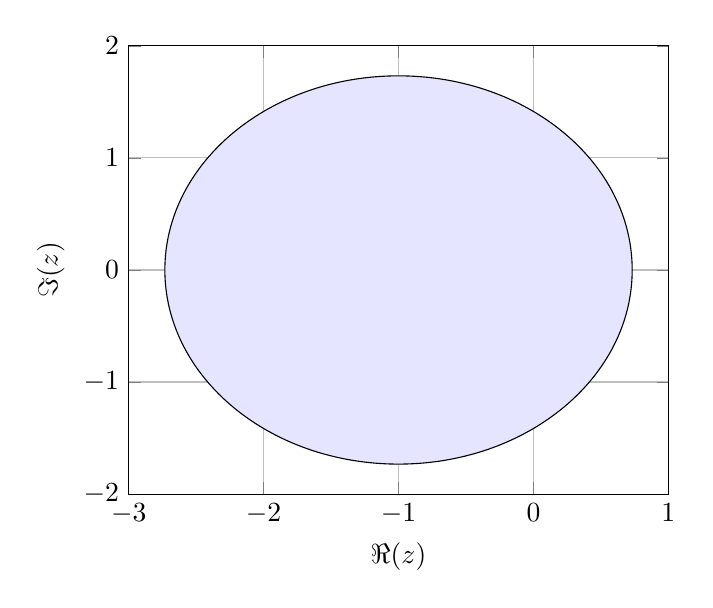
\begin{tikzpicture}
      \begin{axis}[
          xlabel=$\Re(z)$, ylabel=$\Im(z)$,
          xmin=-3, xmax=1, ymin=-2, ymax=2, grid=both]
        \draw[fill=blue!10] (axis cs:-1,0) circle[radius=sqrt(3)];
      \end{axis}
    \end{tikzpicture}
  \end{center}
  This is the circle centered at $(-1,0)$ with radius $\sqrt3$.
\end{proof}


\begin{recommended}
  Let $z,w\in\C$ such that $\overline{z} w \neq 1$.
  Prove that if $|z|=1$ or $|w|=1$, then $\abs{\dfrac{z-w}{1 - \overline{z} w}}=1$.
\end{recommended}
\begin{prf}[by sooshi]
  Let $z$ and $w$ be complex numbers such that $\overline{z} w \neq 1$.
  Suppose that $|z| = 1$ or $|w| = 1$.
  If $z = w$ and $|z| = |w| = 1$, then $\overline{z}w = \overline{z}z = |z|^2 = 1$.
  Therefore, $z \neq w$.

  Now, consider the case when $|z| = 1$. Then,
  \begin{equation*}
    \abs{\frac{z-w}{1 - \overline{z} w}}
    = \frac{|z-w|}{|1 - \overline{z} w|}
    = \frac{|z||z-w|}{|z||1 - \overline{z} w|}
    = \frac{(1)|z-w|}{|z - z\overline{z}w|}
    = \frac{|z-w|}{|z-w|}
    = 1
  \end{equation*}
  Likewise, if $|w| = 1$, then
  \begin{equation*}
    \abs{\frac{z-w}{1 - \overline{z} w}}
    = \frac{|z-w|}{|1 - \overline{z} w|}
    = \frac{|z-w|}{|w\overline{w} - \overline{z} w|}
    = \frac{|z-w|}{|w||\overline{w} - \overline{z}|}
    = \frac{|z-w|}{|w-z|}
    = 1
  \end{equation*}
  since $|w-z| = \abs{-(z-w)} = \abs{-1}|z-w| = |z-w|$, completing the proof.
\end{prf}


\begin{recommended}
  Show that for all complex numbers $z$, $|\Re(z)|+|\Im(z)|\leq\sqrt{2}|z|$.
\end{recommended}
\begin{proof}
  Let $z = r\cis \theta$ be a complex number.
  Then, $|z| = r$, $\Re(z) = r\cos\theta$ and $\Im(z) = r\sin\theta$.
  Due to the symmetry of sine and cosine, instead of taking absolute values,
  we restrict without loss of generality to the first quadrant $0 \leq \theta \leq \frac\pi2$. Now,
  \begin{align*}
    \Re(z) + \Im(z) & = r(\cos\theta + \sin\theta)                                                          \\
                    & = r\sqrt{2}\frac{\sqrt{2}}{2}(\cos\theta + \sin\theta)                                \\
                    & = r\sqrt{2}\left( \frac{\sqrt{2}}{2}\cos\theta + \frac{\sqrt{2}}{2}\sin\theta \right) \\
                    & = r\sqrt{2}\left( \sin\frac\pi4\cos\theta + \cos\frac\pi4\sin\theta \right)           \\
                    & = r\sqrt{2}\sin\left(\frac\pi4 + x\right)                                             \\
                    & \leq r\sqrt{2}(1)                                                                     \\
                    & = \sqrt{2}|z|
  \end{align*}
  completing the proof.
\end{proof}


\begin{recommended}
  Use \emph{De Moivre's Theorem} (DMT) to prove that
  $\sin 4\theta = 4\sin\theta\cos^3\theta - 4\sin^3\theta\cos\theta$ for all $\theta\in\R$.
\end{recommended}
\begin{proof}
  Let $\theta \in \R$ and note that by DMT, we have
  \[ (\cos\theta + i\sin\theta)^4 = \cos 4\theta + i\sin 4\theta \]
  so we may say that $\sin 4\theta = \Im((\cos\theta + i\sin\theta)^4)$.
  Expanding this quantity by hand,
  \begin{align*}
    (\cos\theta + i\sin\theta)^4
     & = (\cos^2 \theta + 2i\cos\theta\sin\theta - \sin^2\theta)^2                                                        \\
     & = \cos^4\theta + \sin^4\theta - 6\cos^2\theta\sin^2\theta + 4i\cos^3\theta\sin\theta - 4i\sin^3\theta\cos\theta    \\
     & = (\cos^4\theta - 6\cos^2\theta\sin^2\theta + \sin^4\theta) + (4\cos^3\theta\sin\theta - 4\sin^3\theta\cos\theta)i
  \end{align*}
  and we have that
  \[ \sin 4\theta = \Im((\cos\theta + i\sin\theta)^4) = 4\cos^3\theta\sin\theta - 4\sin^3\theta\cos\theta \]
  as desired.
\end{proof}


\begin{recommended}
  Let $n\in\N$ and $a,b\in\R$. Show that $z=(a+bi)^n+(a-bi)^n$ is real.
\end{recommended}
\begin{proof}
  Let $n$ be a natural number and $u=a+bi$ be a complex number. Then, $\overline{u}=a-bi$.
  It inductively follows from PCJ4 and the associativity of multiplication
  that $(\overline{u})^n = \overline{u^n}$.

  Now, the fact that $z = u^n + \overline{u^n}$ is real follows immediately from PCJ3.
\end{proof}


\begin{recommended}
  An \emph{$n$-th root of unity} is any complex solution to $z^n=1$.
  Prove that if $w$ is an $n$-th root of unity, $\frac1w$ is also an $n$-th root of unity.
\end{recommended}
\begin{proof}
  Let $n$ be a natural number and $w$ be an $n$-th root of unity, so $w^n = 1$.
  Knowing that $1=\cis0$, the CNRT states that $w = \cis(\frac{2k\pi}{n})$ for some $0 \leq k < n$.

  By PM\C, notice that $w\cis(-\frac{2k\pi}{n}) = \cis(\frac{2k\pi}{n}-\frac{2k\pi}{n}) = \cis 0 = 1$,
  so $\cis(-\frac{2k\pi}{n})$ is the multiplicative inverse $w^{-1}$ of $w$.
  Now, since $\cis$ is $2\pi$-periodic, we have
  \[
    \cis\left(-\frac{2k\pi}{n}\right) = \cis\left(2\pi-\frac{2k\pi}{n}\right)
    = \cis\left(\frac{2n\pi-2k\pi}{n}\right) = \cis\left(\frac{2(n-k)\pi}{n}\right)
  \]
  but since $0 \leq k < n$, we also have that $0 \leq n-k < n$.
  Therefore, by the CNRT, $w^{-1}$ is an $n$-th root of unity.
\end{proof}


\begin{recommended}
  A complex number $z$ is called a \emph{primitive} $n$-th root of unity
  if $z^n=1$ and $z^k \neq 1$ for all $1 \leq k \leq n-1$.
\end{recommended}
\begin{enumerate}[(a)]
  \item For each $n=1,3,5,6$ list all the primitive $n$-th roots of unity.
        \begin{proof}[Solution]
          Recall that $1^x=1$ for any real $x$.
          Applying the CNRT, there are $n$ $n$-th roots of unity, of the form
          \[ z = \cis\left(\frac{2\pi k}{n}\right) \]
          for some integer $0 \leq k < n$.
          Note that 1 is always an $n$-th root of unity but only a primitive first root of unity.
          Therefore, we can ignore the case $k=0$.

          The only primitive 1st root of unity is 1.

          The primitive 3rd roots of unity are
          $\cis \frac{2\pi}{3} = \frac{\sqrt 3}{2} - \frac{1}{2}i$ and
          $\cis \frac{4\pi}{3} = \frac{\sqrt 3}{2} + \frac{1}{2}i$.

          For this, we remain in polar form as calculating sines and cosines of fractions over 5 is \emph{pain}.
          The primitive 5th roots of unity are $\cis 0 = 1$, $\cis \frac{2\pi}{5}$, $\cis \frac{4\pi}{5}$,
          $\cis \frac{6\pi}{5}$, and $\cis \frac{8\pi}{5}$.

          The 6th roots of unity are $\cis \frac{2\pi k}{6} = \cis \frac{\pi k}{3}$.
          However, when $k=2$, $k=3$, and $k=4$, these are also 2nd/3rd roots of unity.
          Thus, the primitive roots of unity are
          $\cis \frac{\pi}{3} = \frac{1}{2} + \frac{\sqrt{3}}{2}i$ and
          $\cis \frac{5\pi}{3} = \frac{1}{2} - \frac{\sqrt{3}}{2}i$.
        \end{proof}
  \item Let $z$ be a primitive $n$-th root of unity. Prove the following statements:
        \begin{enumerate}[i.]
          \item For any $j\in\Z$, $z^j=1$ if and only if $n \mid j$.
                \begin{proof}
                  Let $n$ be a natural number, $j$ be an integer,
                  and $z$ be a primitive $n$-th root of unity so $z^n=1$.
                  Proceed by mutual implication.

                  ($\Rarr$) Suppose $z^j = 1$.
                  By the Division Algorithm, $j = qn + r$ for integers $q$ and $0 \leq r < n$.
                  Then, $1 = z^j = z^{qn+r} = z^{qn}z^r = (z^n)^q z^r = 1^q z^r = z^r$.

                  If $r=0$, then $j = qn$ and $n \mid j$.
                  Otherwise, we have $1 \leq r \leq n-1$ and $z^r = 1$, which is a contradiction
                  to the fact that $z$ is a primitive $n$-th root of unity.

                  Therefore, $r = 0$ and $n \mid j$.

                  ($\Larr$) If $n \mid j$ and $j = nk$ for an integer $k$,
                  then $z^j = z^{nk} = (z^n)^k = 1^k = 1$.
                \end{proof}
          \item For any $m\in\Z$, if $\gcd(m,n)=1$, then $z^m$ is a primitive $n$-th root of unity.
                \begin{prf}[new and improved by sooshi]
                  Let $z$ be a primitive $n$-th root of unity and $m$ an integer coprime to $n$.

                  Suppose for a contradiction that $z^m$ is a $k$-th root of unity for some $1 \leq k < n$.
                  Then, $(z^m)^k = z^{mk} = 1$.
                  From above, this implies that $n \mid mk$ and by CAD, $n \mid k$.
                  However, BBD gives that $n \leq k$, which is a contradiction.

                  Therefore, $z^m$ is a primitive $n$-th root of unity.
                \end{prf}
        \end{enumerate}
\end{enumerate}


\begin{recommended}
  Let $u$ and $v$ be fixed complex numbers.
  Let $\omega$ be a non-real cube root of unity.
  For each $k\in\Z$, define $y_k\in\C$ by the formula \[ y_k = \omega^k u + \omega^{-k}v \]
\end{recommended}
\begin{enumerate}[(a)]
  \item Compute $y_1$, $y_2$, and $y_3$ in terms of $u$, $v$, and $\omega$.
        \begin{proof}[Solution]
          From RP15(a), the only real cube root of unity is 1, so $\omega \neq 1$.
          In fact, $\omega = \cis \frac{n\pi}{3}$ for either $n=2$ or $n=4$.

          If $n=2$, then $\omega^{-1} = \cis \frac{-2\pi}{3} = \cis\frac{4\pi}{3}$.
          If $n=4$, then $\omega^{-1} = \cis \frac{-4\pi}{3} = \cis\frac{2\pi}{3}$.

          However, using the standard form from RP15(a), $\cis\frac{2\pi}{3} = \overline{\cis\frac{4\pi}{3}}$.
          Therefore, $\omega^{-1} = \overline{\omega}$.

          Now, $y_1 = \omega u + \overline{\omega} v$,
          $y_2 = \omega^2 u + \overline{\omega}^2 v$, and
          $y_3 = \omega^3 u + \overline{\omega}^3 v = u + v$.
        \end{proof}
  \item Show that $y_k = y_{k+3}$ for any $k\in\Z$.
        \begin{proof}
          Let $k$ be an integer.
          Then, knowing that both $\omega$ and $\overline{\omega}$ are cube roots of unity,
          \begin{align*}
            y_{k+3} & = \omega^{k+3} u + \overline{\omega}^{k+3} v                      \\
                    & = \omega^k \omega^3 u + \overline{\omega}^k \overline{\omega}^3 v \\
                    & = \omega^k u + \overline{\omega}^k v                              \\
                    & = y_k
          \end{align*}
          completing the proof.
        \end{proof}
  \item Show that for any $k\in\Z$, \[ y_k-y_{k+1} = \omega^k(1-\omega)(u-\omega^{k-1}v) \]
        \begin{proof}
          Let $k$ be an integer. Expand the right-hand side:
          \begin{align*}
            \omega^k(1 - \omega)(u - \omega^{k-1}v)
             & = (\omega^k-\omega^{k+1})(u-\omega^{k-1}v)                         \\
             & = \omega^k u - \omega^{2k+1}v - \omega^{k+1}u + \omega^{2k+2}v     \\
             & = (\omega^k u + \omega^{2k+2}v) - (\omega^{k+1}u + \omega^{2k+1}v)
          \end{align*}
          To simplify, we show that $\omega^{2k+2} = \omega^{-k}$.
          Equivalently, $\omega^{2k+2}\omega^k = \omega^{3k+2} = 1$.
          Let $j = k+1$. Then,
          \[ \omega^{3k+2} = \omega^{3(j-1)+2} = \omega^{3j-1} = (\omega^3)^j \omega^{-1} = 1^j \omega^{-1} = \omega^{-1} \]
          as desired.
          Now, we have $\omega^{2k+2} = \omega^{-k}$ and $\omega^{2k+1} = \omega^{-(k+1)}$ so
          \begin{align*}
            \omega^k(1 - \omega)(u - \omega^{k-1}v)
             & = (\omega^k u + \omega^{2k+2}v) - (\omega^{k+1}u + \omega^{2k+1}v) \\
             & = (\omega^k u + \omega^{-k}v) - (\omega^{k+1}u + \omega^{-(k+1)}v) \\
             & = y_k - y_{k+1} \qedhere
          \end{align*}
        \end{proof}
\end{enumerate}


\section{Challenges}

\begin{challenge}
  Let $z,w\in\C$.
\end{challenge}
\begin{enumerate}[(a)]
  \item Prove that $|z+w| \leq |z| + |w|$.
        \begin{proof}
          This is the Triangle Inequality, for which a geometric proof is provided in Chapter 10.3.
          In short, for complex numbers $z = a+bi$ and $w = c+di$,
          we consider a triangle $\triangle OZW$ with points $O(0,0)$, $Z(a,b)$, and $W(c,d)$ in the complex plane.
          Then, $|z| = \ell_{OZ}$, $|w| = \ell_{OW}$, and $|z+w| = \ell_{ZW}$.
          The length of one side of a triangle cannot exceed the sum of the lengths of the other two sides.

          Equivalently, $\ell_{ZW} \leq \ell_{OZ} + \ell_{OW}$.
        \end{proof}
  \item Prove that $\abs{|z| - |w|} \leq |z-w| \leq |z|+|w|$.
        \begin{proof}
          Let $z$ and $w$ be complex numbers.
          We prove the inequalities separately.

          We apply the Triangle Inequality with $z$ and $-w$.
          Then, $|z + (-w)| \leq |z| + |-w|$ but $|-w| = |-1||w| = |w|$ by PM4,
          so we have $|z-w| \leq |z| + |w|$.

          Now, notice that $|z| = |(z-w) + w| \leq |z-w| + |w|$ so $|z| - |w| \leq |z-w|$.

          Likewise, $|w| = |(w-z) + z| \leq |w-z| + |z|$ so $|z| - |w| \geq -|w-z|$.

          Like the absolute value in \R, we have by PM4 $|w-z| = |-1||z-w| = 1|z-w| = |z-w|$,
          so if we combine the above two inequalities, we have $\abs{|z| - |w|} \leq |z-w|$.

          Equivalently, using the same triangle from above, this follows from the fact that
          any one side of a triangle is longer than the difference of the other two sides.
        \end{proof}
\end{enumerate}

\begin{challenge}
  Let $a,b,c\in\C$.
  Show that if $\dfrac{b-a}{a-c} = \dfrac{a-c}{c-b}$ then $|b-a| = |a-c| = |c-b|$.
\end{challenge}

\begin{challenge}
  Let $n \geq 2$ be an integer. Prove that
  \[ \sum_{k=0}^{n-1}\cos\left(\frac{2k\pi}{n}\right)=0=\sum_{k=0}^{n-1}\sin\left(\frac{2k\pi}{n}\right) \]
\end{challenge}
\begin{prf}[with help from Ainsley, Kenson, Mabel]
  Let $n \neq 1$ be a natural number.
  Then, we have that the $n$-th roots of unity are given by
  \[ \cos(\frac{2k\pi}{n}) + i \sin(\frac{2k\pi}{n}) \]
  for $k = 0,1,2,\ldots,n-1$.
  Let $z$ be the sum of the $n$-th roots of unity. Then,
  \[ z = \sum_{k=0}^{n-1}\left(\cos(\frac{2k\pi}{n}) + i\sin(\frac{2k\pi}{n})\right) \]
  The conclusion can equivalently be stated as that $\Re(z) = 0$ and $\Im(z) = 0$.
  The only complex number that satisfies this is $z = 0$.

  Now, let $a = \cos(\frac{2\pi}{n}) + i\sin(\frac{2\pi}{n})$, the root of unity with $k = 1$.
  Then, we have that each root of unity is given by $a^j$ for $j = 1,2,\ldots,n$.
  Since $n \neq 1$, $a = \cis\frac{2\pi}{n} \neq 1$ and $z = 1 + a + a^2 + \cdots + a^{n-1}$.

  Recall that the polynomial $a^n - 1$ for $n \geq 2$ factors as
  $(a-1)(a^{n-1} + a^{n-2} + \cdots + a^2 + a + 1)$.
  It follows that $a^n - 1 = 1-1 = 0$ and $0 = (a-1)z$ so, from above, $a \neq 1$ so $z = 0$.
\end{prf}

\chapter{Polynomials}

\section{Warm-Up Exercises}

\begin{warmup}
  Find a real cubic polynomial whose roots include 1 and $i$.
\end{warmup}
\begin{proof}[Solution]
  Apply the Factor Thorem to create $f(x) = (x-1)(x-i)(x-r)$.
  To ensure the polynomial is real, make $(x-r)$ the conjugate of $(x-i)$, i.e., $r=-i$.
  Then, $f(x) = (x-1)(x^2+1) = x^3 - x^2 + x - 1$.
\end{proof}


\begin{warmup}
  Divide $f(x)=x^3+x^2+x+1$ by $g(x)=x^2+4x+3$ to find the quotient $q(x)$ and remainder $r(x)$
  that satisfy the requirements of the \emph{Division Algorithm for Polynomials} (DAP)
\end{warmup}
\begin{proof}[Solution]
  Perform polynomial long division:
  \[ \polylongdiv{x^3+x^2+x+1}{x^2+4x+3} \]
  and conclude that $q(x) = 10x + 10$ and $r(x) = x - 3$.
\end{proof}


\section{Recommended Problems}

\begin{recommended}
  Let $z\in\C$. Prove that $(x-z)(x-\overline{z}) \in \R[x]$.
\end{recommended}
\begin{proof}
  Let $z$ be a complex number.
  Expand the product to obtain
  \begin{align*}
    (x-z)(x-\overline{z}) & = x^2 - zx - \overline{z}x + z\overline{z}  \\
                          & = x^2 - (z + \overline{z})x + z\overline{z}
  \end{align*}
  which is a polynomial in $x$ with coefficients $1$, $-(z+\overline{z})$, and $z\overline{z}$.
  Clearly, $1 \in \R$.
  From PCJ3, we have $z+\overline{z} = 2\Re z$ so $-(z+\overline{z}) = -2 \Re z \in \R$.
  Also, from PM3, $z\overline{z}=|z|^2 \in \R$.
  Therefore, the polynomial is a member of $\R[x]$.
\end{proof}


\begin{recommended}
  Prove that there exists a polynomial in $\Q[x]$ with the root $2-\sqrt 7$.
\end{recommended}
\begin{proof}
  We propose $f(x) = x^2 - 4x - 3 \in \Q[x]$.
  \[ f(2-\sqrt{7}) = (2-\sqrt7)^2 - 4(2-\sqrt7) - 3 = 11 - 4\sqrt7 - 8 + 4\sqrt7 - 3 = 0 \qedhere \]
\end{proof}


\begin{recommended}
  For each of the following polynomials $f(x) \in \F[x]$,
  write $f(x)$ as a product of irreducible polynomials in $\F[x]$.
\end{recommended}
\begin{enumerate}[(a)]
  \item $x^2 - 2x + 2 \in \C[x]$
        \begin{proof}[Solution]
          We apply the quadratic formula to find that $x = \frac{2+\sqrt{-4}}{2} = 1+i$.
          Then, we also have $x = 1-i$ as a solution.
          Therefore, we may write in irreducible polynomials $f(x)=(x-1-i)(x-1+i)$.
        \end{proof}
  \item $x^2 + (-3i + 2)x - 6i \in \C[x]$
        \begin{proof}[Solution]
          By inspection, $x=-2$ is a root.
          Divide by $g(x)=x+2$ to obtain $q(x)=x-3i$.
          Therefore, we write in irreducible polynomials $f(x)=(x+2)(x-3i)$.
        \end{proof}
  \item $2x^3 - 3x^2 + 2x + 2 \in \R[x]$
        \begin{proof}[Solution]
          The RRT gives $x=1,-1,2,-2,\frac12,-\frac12$ as candidates for roots of $f$.
          We find that $f(-\frac12)=0$, so we divide by $g(x)=2x+1$ to find $q(x)=x^2-2x+2$.
          Now, the discriminant of $q$ is negative, so it has no real solutions and is irreducible in $\R[x]$.
          Therefore, we write $f(x)=(2x+1)(x^2-2x+2)$.
        \end{proof}
  \item $3x^4 + 13x^3 + 16x^2 + 7x + 1 \in \R[x]$
        \begin{proof}[Solution]
          By inspection, $x=-1$ is a root.
          Divide by $g(x)=x+1$ to obtain $q(x)=3x^3+10x^2+6x+1$.
          To find roots of this cubic, the RRT gives candidates $x=1,-1,\frac13,-\frac13$.
          In fact, $q(-\frac13)=0$.
          Dividing $q(x)$ by $(3x+1)$, we obtain the factor $(x^2+3x+1)$.
          The discriminant of this quadratic is positive
          and it has roots $-\frac32 \pm \frac{\sqrt{5}}{2}$.
          Therefore, $f(x) = (x+1)(3x+1)(x-\frac32+\frac{\sqrt{5}}{2})(x-\frac32-\frac{\sqrt{5}}{2})$.
        \end{proof}
  \item $x^4 + 27x \in \C[x]$
        \begin{proof}[Solution]
          Factor: $f(x) = x(x^3 + 27)$.
          The roots are $x=0$ and $x=\sqrt[3]{-27}=3\sqrt[3]{-1}$.
          By the CNRT, the cube roots of $-1$ are $-1$,
          $\frac12+\frac{\sqrt{3}}2i$, and $\frac12-\frac{\sqrt{3}}2i$. Therefore,
          \[ f(x) = x(x+3)\qty(x-\frac{3}{2}-\frac{3\sqrt{3}}{2}i)\qty(x-\frac{3}{2}+\frac{3\sqrt{3}}{2}i) \qedhere \]
        \end{proof}
\end{enumerate}


\begin{recommended}
  Let $g(x)=x^3+bx^2+cx+d\in\C[x]$ be a monic cubic polynomial.
  Let $z_1$, $z_2$, and $z_3$ be three roots of $g(x)$ such that
  \[ g(x) = (x-z_1)(x-z_2)(x-z_3) \]
  Prove that \begin{align*}
    z_1 + z_2 + z_3          & = -b \\
    z_1z_2 + z_2z_3 + z_3z_1 & = c  \\
    z_1z_2z_3                & = -d
  \end{align*}
\end{recommended}
\begin{proof}
  Let $g$ be a monic cubic polynomial over \C, where $z_1$, $z_2$, and $z_3$ are its roots.
  Then, by CPN, $g(x) = x^3 + bx^2 + cx + d = (x-z_1)(x-z_2)(x-z_3)$ for some coefficients $b,c,d\in\C$.
  We expand using standard arithmetic:
  \begin{align*}
    x^3 + bx^2 + cx + d & = (x-z_1)(x-z_2)(x-z_3)                                                    \\
                        & = (x^2 - xz_1 - xz_2 + z_1z_2)(x-z_3)                                      \\
                        & = x^3 - x^2z_1 - x^2z_2 + z_1z_2x - x^2z_3 - z_1z_3x - z_2z_3x - z_1z_2z_3 \\
                        & = x^3 - (z_1 + z_2 + z_3)x^2 + (z_1z_2 + z_2z_3 + z_3z_1)x - z_1z_2z_3
  \end{align*}
  Recall that two polynomials are defined to be equal if and only if their coefficients agree.
  Therefore, $b = -(z_1+z_2+z_3)$, $c = z_1z_2 + z_2z_3 + z_3z_1$, and $d = -z_1z_2z_3$
  and the conclusion immediately follows.
\end{proof}


\begin{recommended}
  Using the Rational Roots Theorem, prove that $\sqrt 3 + \sqrt 7$ is irrational.
\end{recommended}
\begin{proof}
  Let $a = \sqrt 3 + \sqrt 7$.
  Then, $a^2 = 10 + 2\sqrt{21}$ and $a^2 - 10 = 2\sqrt{21}$.
  Squaring again, $a^4 - 20a^2 + 100 = 84$, i.e., $a^4 + 20a^2 - 16 = 0$.

  Now, we can let $f(x) = x^4 - 20x^2 + 16$ such that $f(a) = 0$.
  The RRT gives that rational roots of $f$ are of the form $p/q$ with coprime integers $p$ and $q$
  where $p \mid 16$ and $q \mid 1$. The divisors of 1 are $\pm1$ and of 16 are $\pm1,\pm2,\pm4,\pm8,\pm16$.
  Note that $f$ is even, so we need only test $x=1,\frac12,\frac14,\frac18,\frac1{16}$.

  Now, $f(1)=5$, $f(\frac12)=-\frac{175}{16}$, $f(\frac14)=-\frac{3775}{256}$,
  $f(\frac18)=-\frac{64255}{4096}$, and $f(\frac1{16})=-\frac{1043455}{65536}$.

  Therefore, $f$ has no rational roots. However, $a$ is a root of $f$, therefore, $a$ is irrational.
\end{proof}


\begin{recommended}
\end{recommended}
\begin{enumerate}[(a)]
  \item Prove that for every prime $p$, there exists a polynomial $f(x)$ over $\Z_p$,
        of degree $p$, such that every element of $\Z_p$ is a root of $f(x)$.
        \begin{proof}
          Let $p$ be a prime number.
          Then, $\Z_p$ is a field.
          For each element $[n] \in \Z_p$, there is a linear factor $([1]x - [n]) \in \Z_p[x]$.
          The product of polynomials is well-defined and is a polynomial, so we may say that
          the polynomial $f(x) \in \Z_p[x]$ \[ f(x) = \prod_{[i] \in \Z_p}([1]x - [i]) \]
          has $p$ roots corresponding to each of the $p$ elements in $\Z_p$.
          The degree of a product is the sum of the degrees of the factors,
          but each factor is linear with degree 1 so the sum is simply $p$.
        \end{proof}
  \item Prove that for every prime $p$, there exists a polynomial $f(x)$ over $\Z_p$,
        of degree $p$, which has no roots in $\Z_p$.
        \begin{proof}
          Let $p$ be a prime number and let $g(x)$ be the polynomial from (a) above for $p$.
          Then, $g(x) \equiv 0 \pmod p$ for any $x \in \Z_p$.
          Therefore, $g(x) \not\equiv 1 \pmod p$ for any $x$ and we may say the polynomial
          $f(x) = g(x) - 1$ has no solutions in $\Z_p$.
        \end{proof}
\end{enumerate}


\begin{recommended}
  Suppose $f(x) = a_n x^n + a_{n-1} x^{n-1} + \cdots + a_1 x + a_0 \in \C[x]$ with degree $n$.
  We say $f(x)$ is \emph{palindromic} if the coefficients $a_j$ satisfy
  \[ a_{n-j} = a_j \quad \text{for all} \quad 0 \leq j \leq n \]
  Prove that
\end{recommended}
\begin{enumerate}[(a)]
  \item If $f(x)$ is a palindromic polynomial and $c \in \C$ is a root of $f(x)$,
        then $c$ must be non-zero, and $\frac{1}{c}$ is also a root of $f(x)$.
        \begin{proof}
          Let $f(x) \in \C[x]$ be a palindromic polynomial with coefficients $a_n$ and root $c$ so
          \[ 0 = a_n c^n + a_{n-1} c^{n-1} + \cdots + a_1 c + a_0 \]
          Since $f(x)$ has degree $n$, $a_n \neq 0$.
          As $f(x)$ is palindromic, $a_0 \neq 0$.
          Suppose that $c = 0$ and substitute above.
          We have that $a_0 = 0$, which is a contradiction.
          Therefore, $c \neq 0$.
          Now, multiplying through by $c^{-n}$, we have
          \[ 0 = a_n + a_{n-1} c^{-1} + \cdots + a_1 c^{-n+1} + a_0 c^{-n} \]
          but since $f(x)$ is palindromic we substitute $a_{n-j}$ for $a_j$ and write
          \[ 0 = a_0 + a_1\left(\frac1c\right) + \cdots + a_{n-1}\left(\frac1c\right)^{n-1} + a_n \left(\frac1c\right)^n \]
          But this is just saying $f(\frac1c) = 0$, that is, $\frac1c$ is a root of $f(x)$.
        \end{proof}
  \item If $f(x)$ is a palindromic polynomial of odd degree, then $f(-1) = 0$.
        \begin{proof}
          Let $f(x)$ be a palindromic polynomial in \C{} with odd degree $n$ and coefficients $a_n$.
          Since $n$ is odd, we have $n=2k+1$ for some integer $k$. Then,
          \[ f(-1) = a_{2k+1} (-1)^{2k+1} + a_{2k} (-1)^{2k} + \cdots + a_1 (-1) + a_0 \]
          and we apply the fact that $a_{n-j} = a_j$ for all $0 \leq j \leq k$ to get
          \[ f(-1) = a_0 (-1)^{2k+1} + a_1 (-1)^{2k} + \cdots + a_k (-1)^{k+1} + a_k (-1)^k + \cdots + a_1 (-1) + a_0 \]
          Notice that there are an even ($n+1 = 2k+2$) number of terms.
          We pair them by common coefficients.
          Let $0 \leq i \leq k$.
          Then, the coefficient $a_i$ appears in the terms $a_i (-1)^{2k+1-i}$ and $a_i (-1)^{i}$.
          The difference in the powers is $2(k-i)+1$, an odd number.
          Therefore, one is even and the other is odd.
          Suppose WLOG that $i$ is even.
          Then, $a_i (-1)^{2k+1-i} = -a_i$ and $a_i (-1)^{i} = a_i$.

          It follows that each term cancels its palindromic term, and the resulting sum is 0.
        \end{proof}
  \item If $\deg f = 1$ and $f(x)$ is a monic, palindromic polynomial, then $f(x) = x+1$.
        \begin{proof}
          Let $f(x)$ be a first-degree polynomial in \C, that is, $f(x) = a_1x + a_0$.
          Since $f(x)$ is monic, its leading coefficient $a_1$ is 1.
          However, since $f(x)$ is palindromic, $a_{\deg f - 1} = = a_{1-1} = a_0 = 1$ as well.
          Therefore, $f(x) = x + 1$.
        \end{proof}
\end{enumerate}


\section{Challenge}

\begin{challenge}
  We call a polynomial primitive if the greatest common divisor of all of its coefficients is 1.
  Show that the product of two primitive polynomials is again primitive.
\end{challenge}

\end{document}

\end{document}
